\chapter{Reporting}

\section{Pengenalan BIRT (Business Intelligence Reporting Tool)}

\textbf{BIRT (Business Intelligence Reporting Tool)} adalah alat pelaporan dan visualisasi data yang dirancang untuk membantu organisasi dalam menghasilkan laporan bisnis yang terstruktur dan terperinci. BIRT adalah bagian dari proyek open-source Eclipse yang menyediakan platform yang kuat untuk membangun laporan yang dapat disematkan dalam aplikasi Java atau berbasis web.

BIRT dikembangkan dengan tujuan untuk memenuhi kebutuhan bisnis akan \textit{business intelligence} (BI), yakni kemampuan untuk mengumpulkan, menganalisis, dan menyajikan data dalam format yang mudah dipahami. Sebagai alat yang banyak digunakan dalam lingkungan perusahaan, BIRT mampu menghasilkan berbagai jenis laporan, seperti:

\begin{itemize}
	\item Laporan tabel dan grafik.
	\item Laporan interaktif yang memungkinkan pengguna untuk menggali data lebih dalam (\textit{drill-down reports}).
	\item Dashboard untuk menampilkan metrik kinerja utama (KPI).
\end{itemize}

\subsection{Fitur Utama}

Beberapa fitur utama dari BIRT meliputi:

\begin{itemize}
	\item \textbf{Desainer Laporan Visual}: BIRT menyediakan antarmuka visual yang memungkinkan pengguna untuk membuat laporan dengan cara seret dan lepas (\textit{drag-and-drop}), sehingga mempermudah pembuatan laporan kompleks tanpa perlu keterampilan pemrograman yang mendalam.
	\item \textbf{Komponen Data Terintegrasi}: BIRT mendukung berbagai sumber data, termasuk \textit{relational databases} (seperti MySQL, Oracle, PostgreSQL), file CSV, hingga \textit{web services}. Dengan konektor bawaan, BIRT dapat dengan mudah menarik data dari sumber-sumber ini.
	\item \textbf{Kemampuan Ekspor}: Laporan yang dihasilkan BIRT dapat diekspor dalam berbagai format, seperti PDF, Excel, dan HTML, yang memudahkan distribusi laporan ke berbagai audiens.
	\item \textbf{Kustomisasi dan Ekstensibilitas}: BIRT memungkinkan pengguna untuk menambahkan skrip atau kode khusus, seperti JavaScript atau Java, untuk memperluas fungsionalitas laporan.
\end{itemize}

\subsection{Arsitektur BIRT}

Secara arsitektural, BIRT terdiri dari dua komponen utama:

\begin{enumerate}
	\item \textbf{Report Designer}: Komponen ini menyediakan lingkungan pengembangan untuk mendesain laporan. Dalam Eclipse IDE, pengguna dapat membuat laporan, mendefinisikan \textit{data source}, menambahkan elemen visual, dan melakukan konfigurasi lainnya.
	\item \textbf{Report Engine}: Setelah laporan selesai dibuat, \textit{Report Engine} bertugas untuk menghasilkan laporan tersebut sesuai dengan \textit{format} dan data yang diinginkan. Komponen ini dapat disematkan dalam aplikasi web atau desktop.
\end{enumerate}

\section{Langkah-Langkah Penggunaan BIRT}

\subsection{Membuat Report File}

Berikut adalah langkah-langkah untuk membuat \textit{Report File} di BIRT, yang akan menyajikan data dalam format laporan.

\begin{enumerate}
	\item Klik kanan pada folder kerja di Eclipse, pilih \textbf{New > Others}. \\
	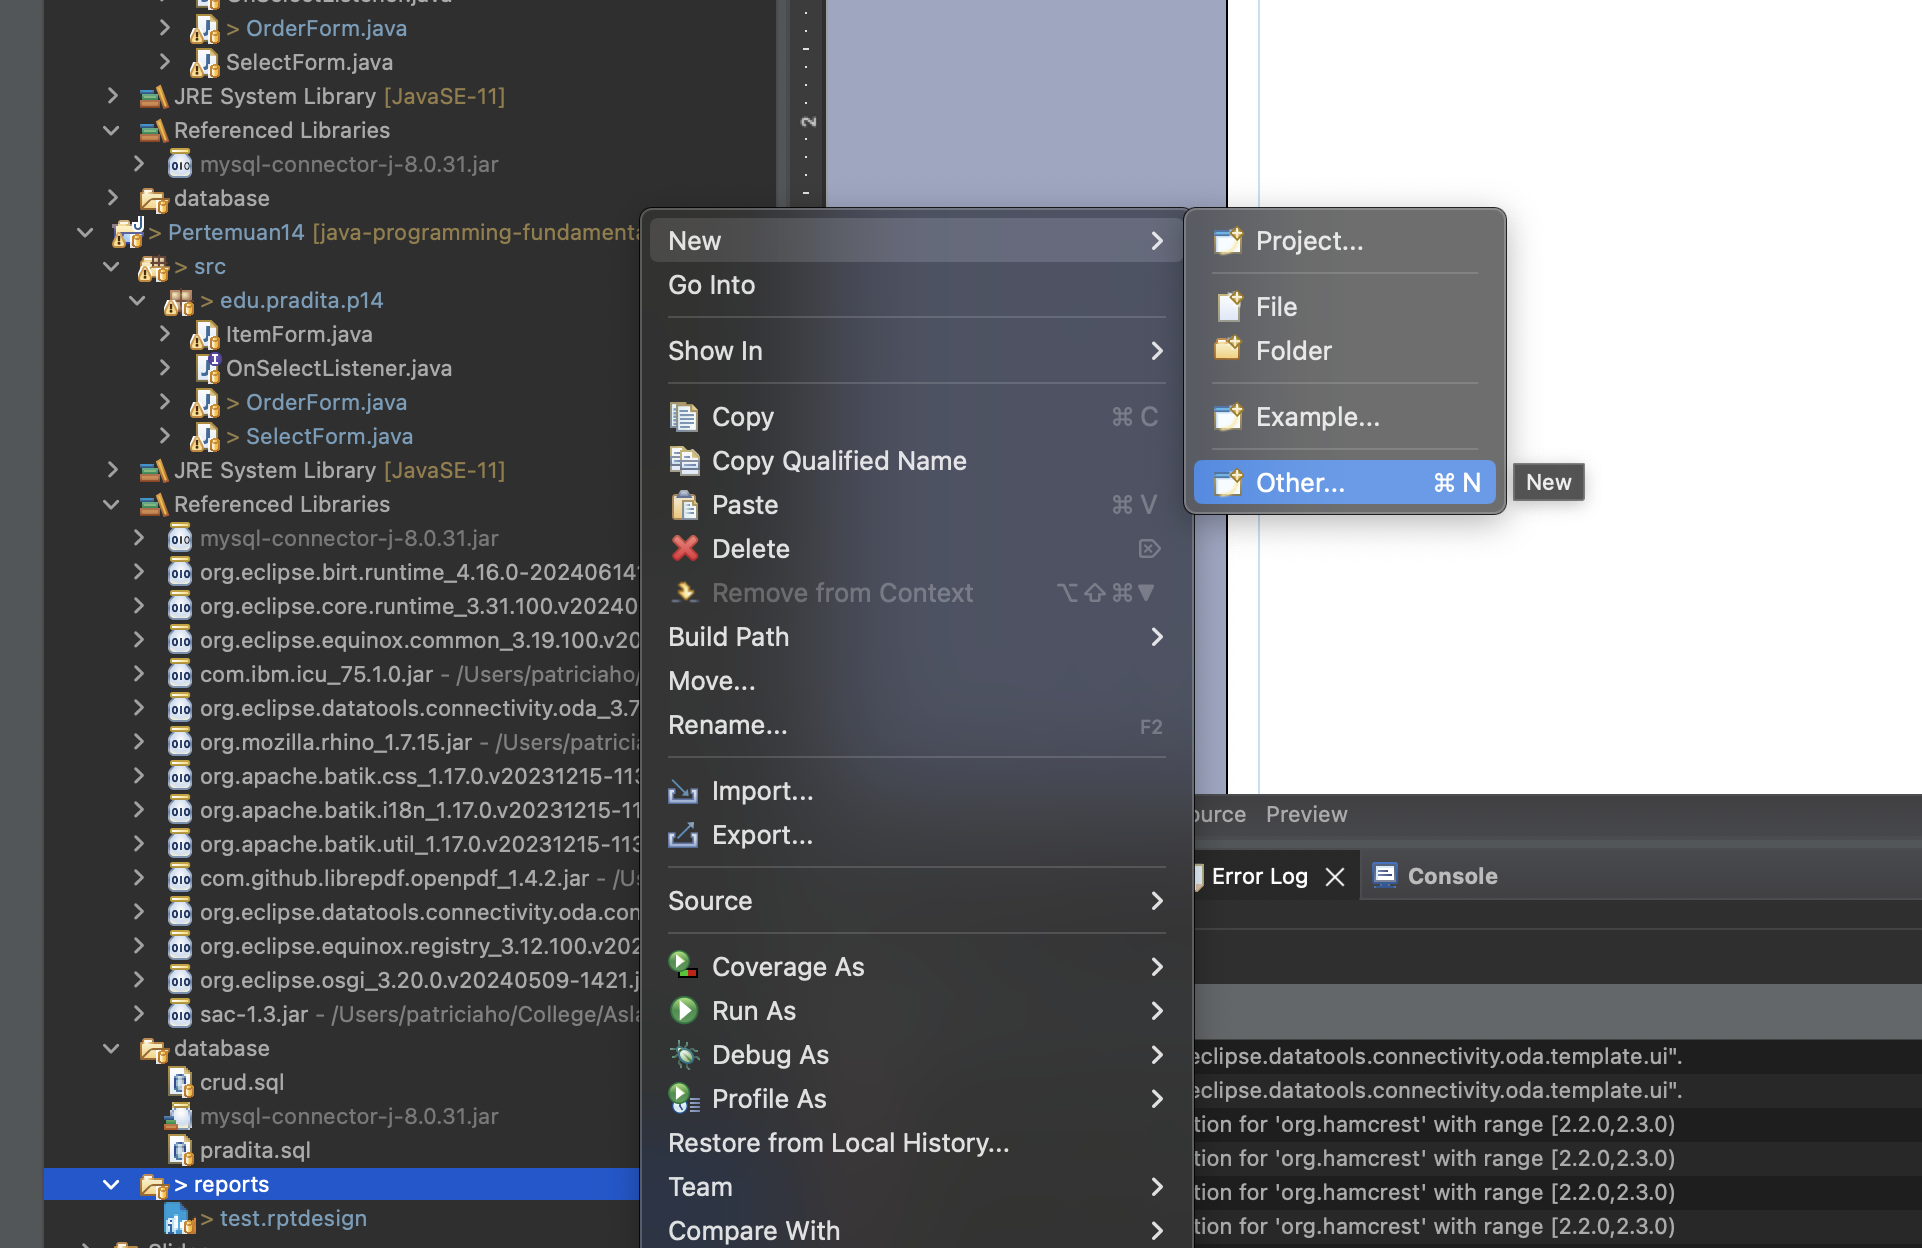
\includegraphics[width=0.8\textwidth]{assets/pertemuan14/New-Report/birt-new-other-file.png}
	
	\item Expand folder Business Intelligence and Reporting Tool, dan pilih Report \\
	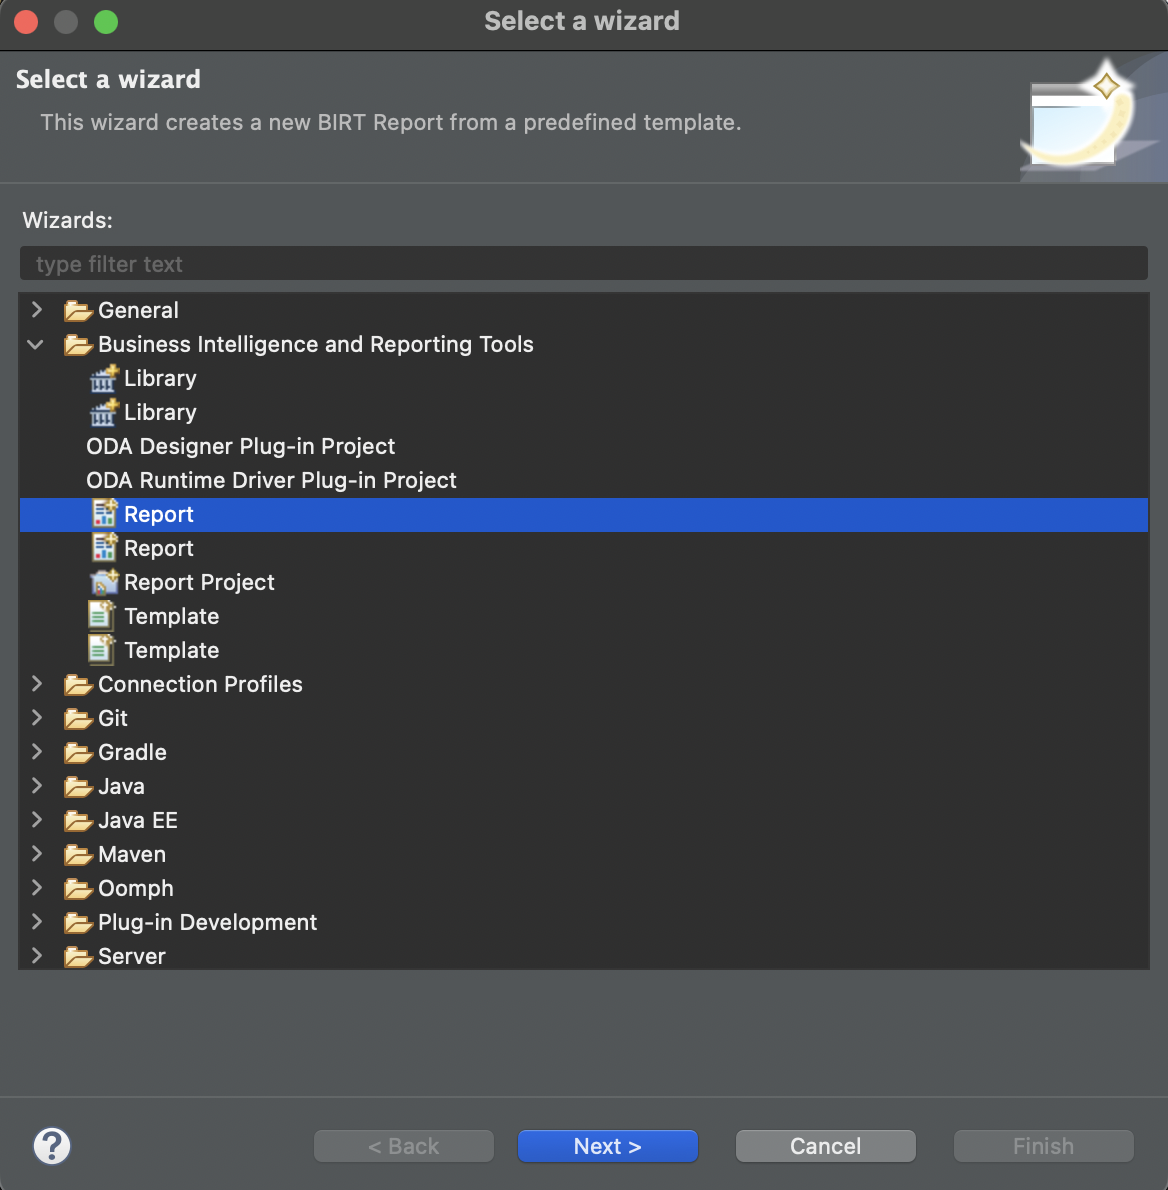
\includegraphics[width=0.5\textwidth]{assets/pertemuan14/New-Report/birt-select-for-wizard-report.png}
	
	\item Beri nama pada \textit{Report File} Anda, lalu klik \textbf{Next}. \\
	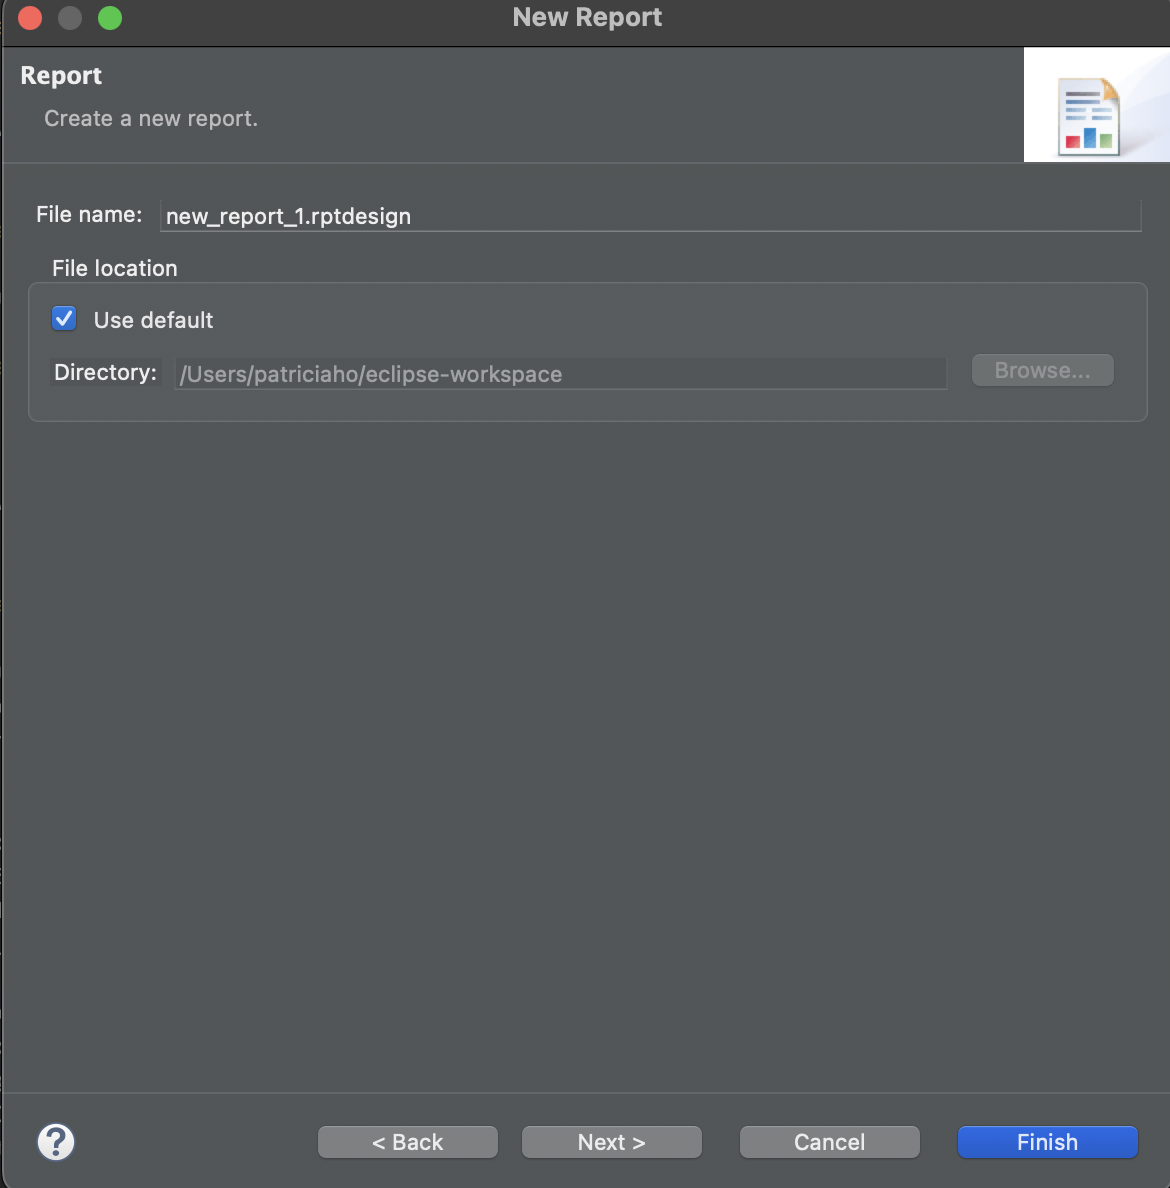
\includegraphics[width=0.5\textwidth]{assets/pertemuan14/New-Report/birt-create-new-report.png}
	
	\item Pilih \textbf{Blank Report} atau template yang sesuai dengan kebutuhan Anda, lalu klik \textbf{Finish}.
\end{enumerate}


\subsection{Menambah Data Source}

\textit{Data Source} adalah sumber data yang menghubungkan BIRT dengan database. Untuk membuat \textit{Data Source} baru, ikuti langkah-langkah berikut:

\begin{enumerate}
	\item Pada panel \textit{Data Explorer}, klik kanan pada \textbf{Data Sources} dan pilih \textbf{New Data Source}. \\
	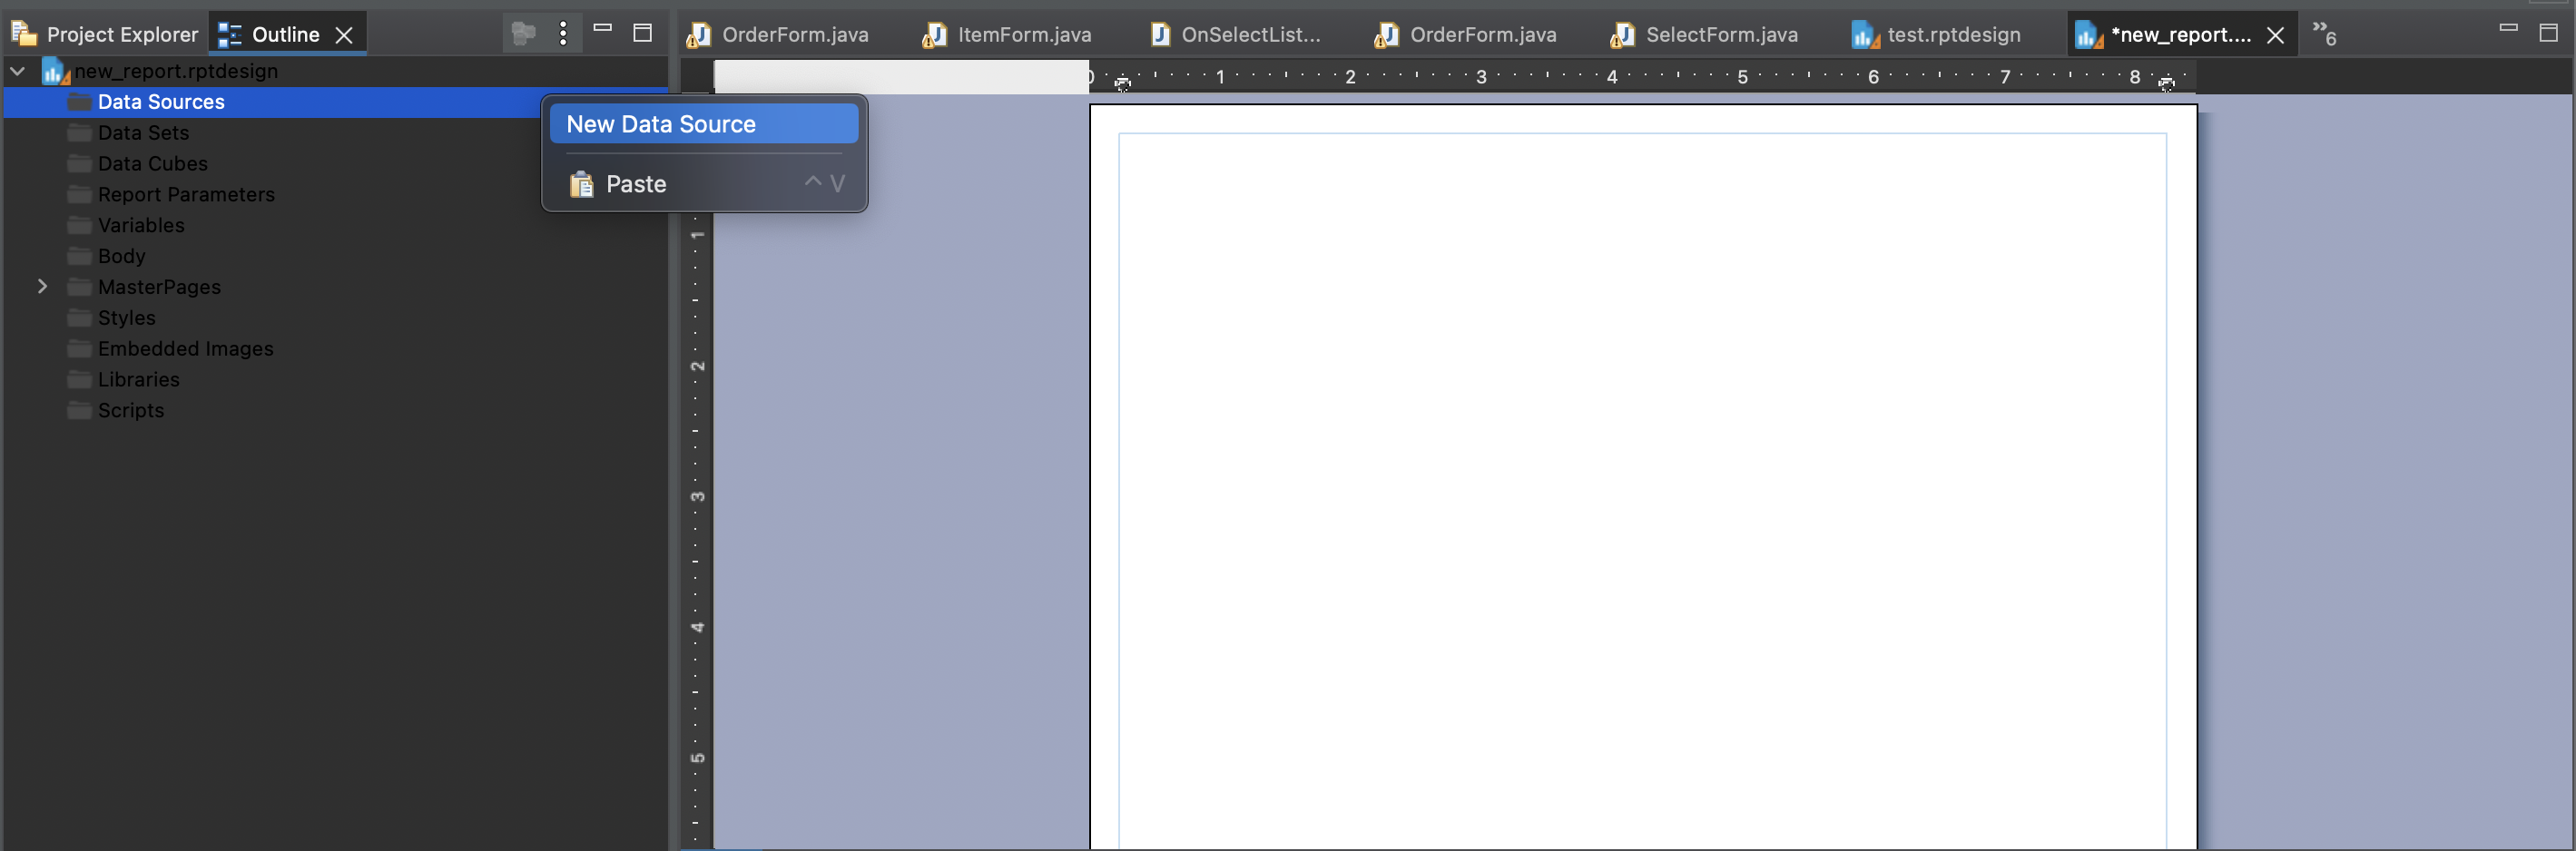
\includegraphics[width=1\textwidth]{assets/pertemuan14/Data-Source/birt-pre-new-data-source.png}
	
	\item Beri nama pada \textit{Data Source} Anda, lalu pilih \textbf{JDBC Data Source} sebagai tipe koneksi dan klik \textbf{Next}. \\
	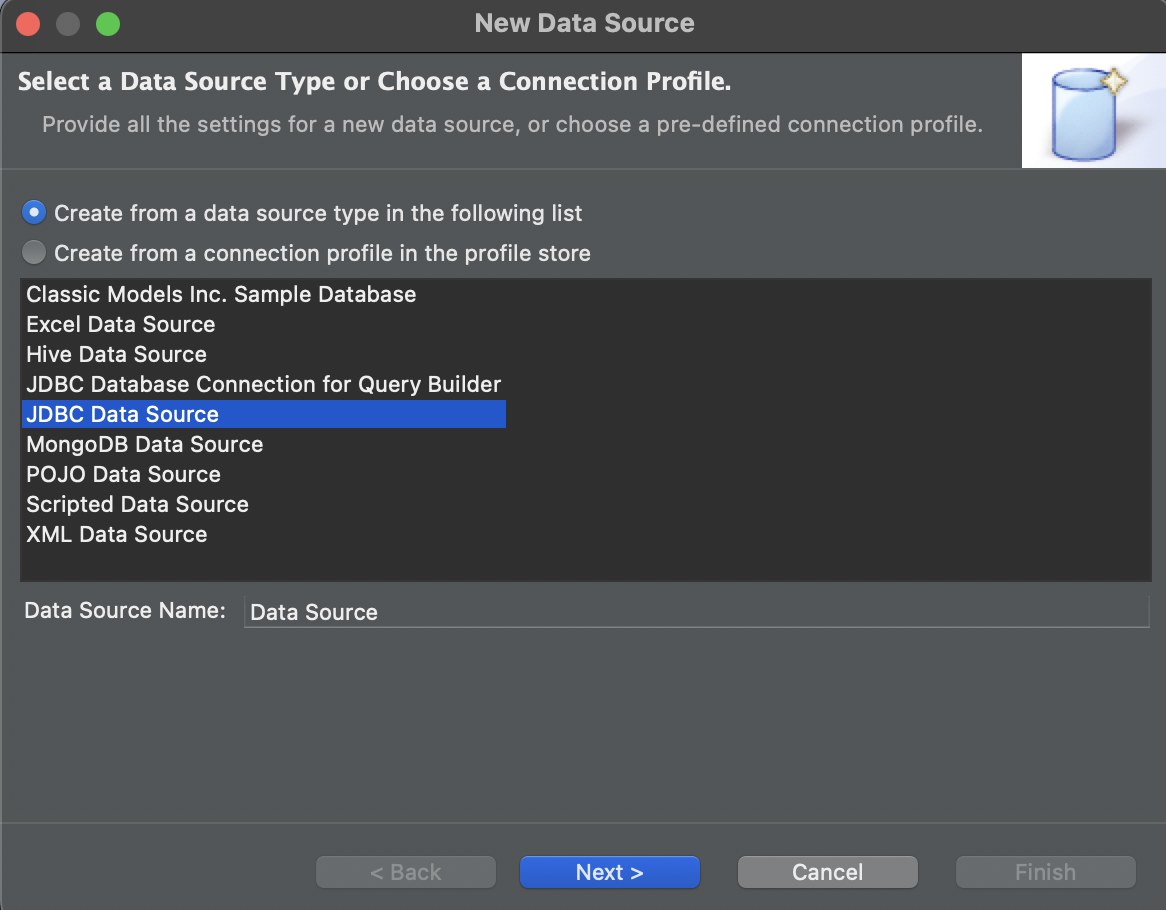
\includegraphics[width=0.5\textwidth]{assets/pertemuan14/Data-Source/birt-select-data-source-type.png}
	
	\item Masukkan informasi koneksi JDBC, termasuk:
	\begin{itemize}
			\item \textbf{Driver Class}: Masukkan nama kelas driver JDBC (misalnya, \texttt{com.mysql.cj.jdbc.Driver} untuk MySQL).\\
			Bila tidak ada nama driver {com.mysql.cj.jbdc.Driver}, ikuti cara berikut:
			
			\begin{itemize}
					\item Pilih Manage Drivers...
					\item Pada tampilan Manage JBDC Drivers dan section JAR Files, pastikan sudah ada mysql-connector. Bila belum, pilih add.
					\item Klik Ok
			\end{itemize}  
			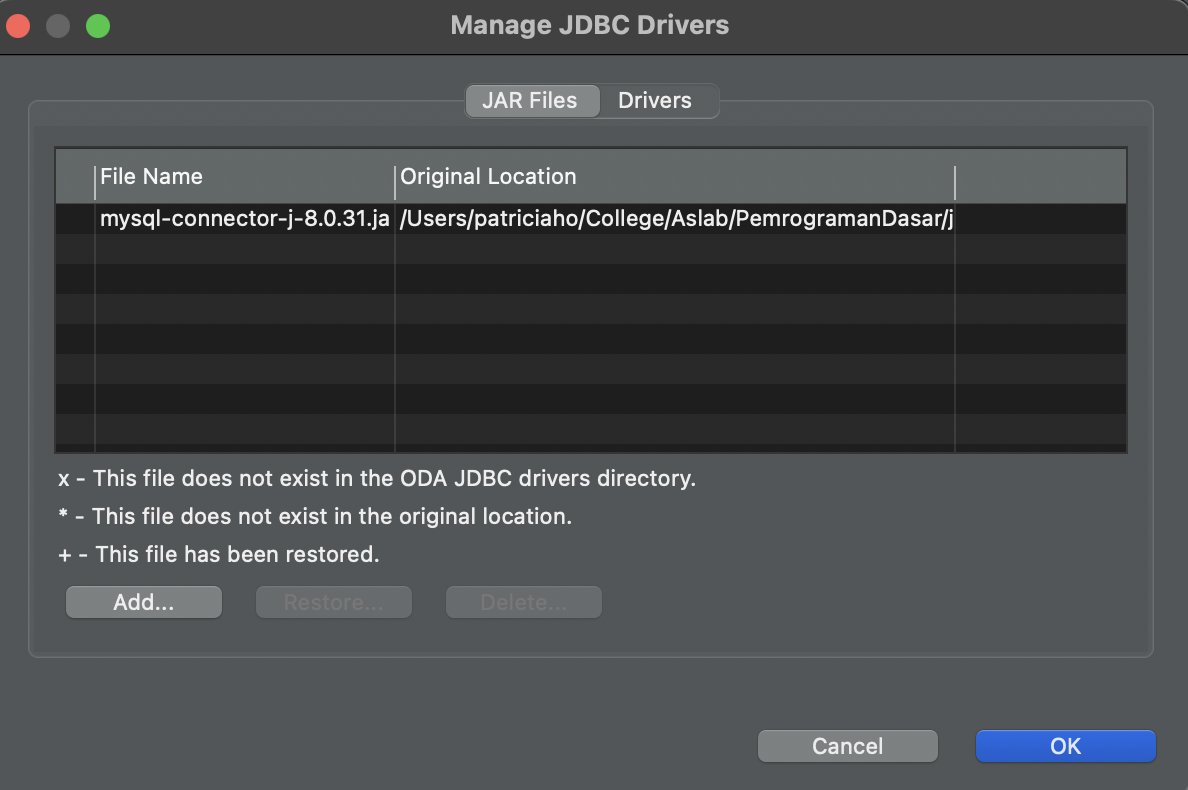
\includegraphics[width=0.5\textwidth]{assets/pertemuan14/Data-Source/birt-manage-jbdc-drivers.png}
			
			\item \textbf{JDBC URL}: Masukkan URL koneksi JDBC yang sesuai untuk database Anda, misalnya:
			\begin{verbatim}
					jdbc:mysql://localhost:3306/nama_database
				\end{verbatim} 
			\item \textbf{Username} dan \textbf{Password}: Masukkan kredensial untuk mengakses database Anda.
		\end{itemize} 
		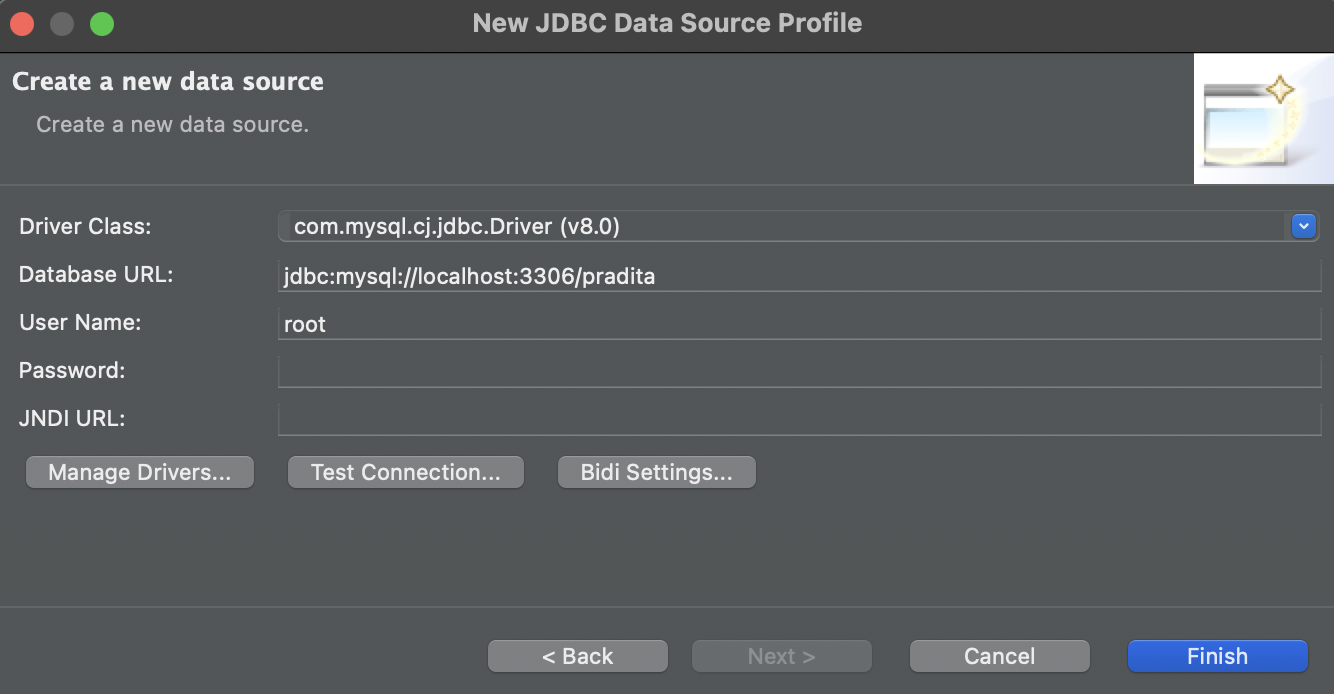
\includegraphics[width=0.5\textwidth]{assets/pertemuan14/Data-Source/birt-create-new-data-source.png}
	
	
	\item Klik \textbf{Test Connection} untuk memastikan koneksi berhasil.
	\item Jika koneksi berhasil, klik \textbf{Finish} untuk menyimpan \textit{Data Source}.
\end{enumerate}




\subsection{Menambah Data Set dari JDBC}

\textit{Data Set} adalah kumpulan data yang diambil dari suatu \textit{Data Source}. Langkah-langkah berikut menjelaskan cara menambah \textit{Data Set} menggunakan koneksi JDBC (Java Database Connectivity).

\begin{enumerate}
	\item Pada panel \textit{Data Explorer}, klik kanan pada \textbf{Data Sets} dan pilih \textbf{New Data Set}. \\
	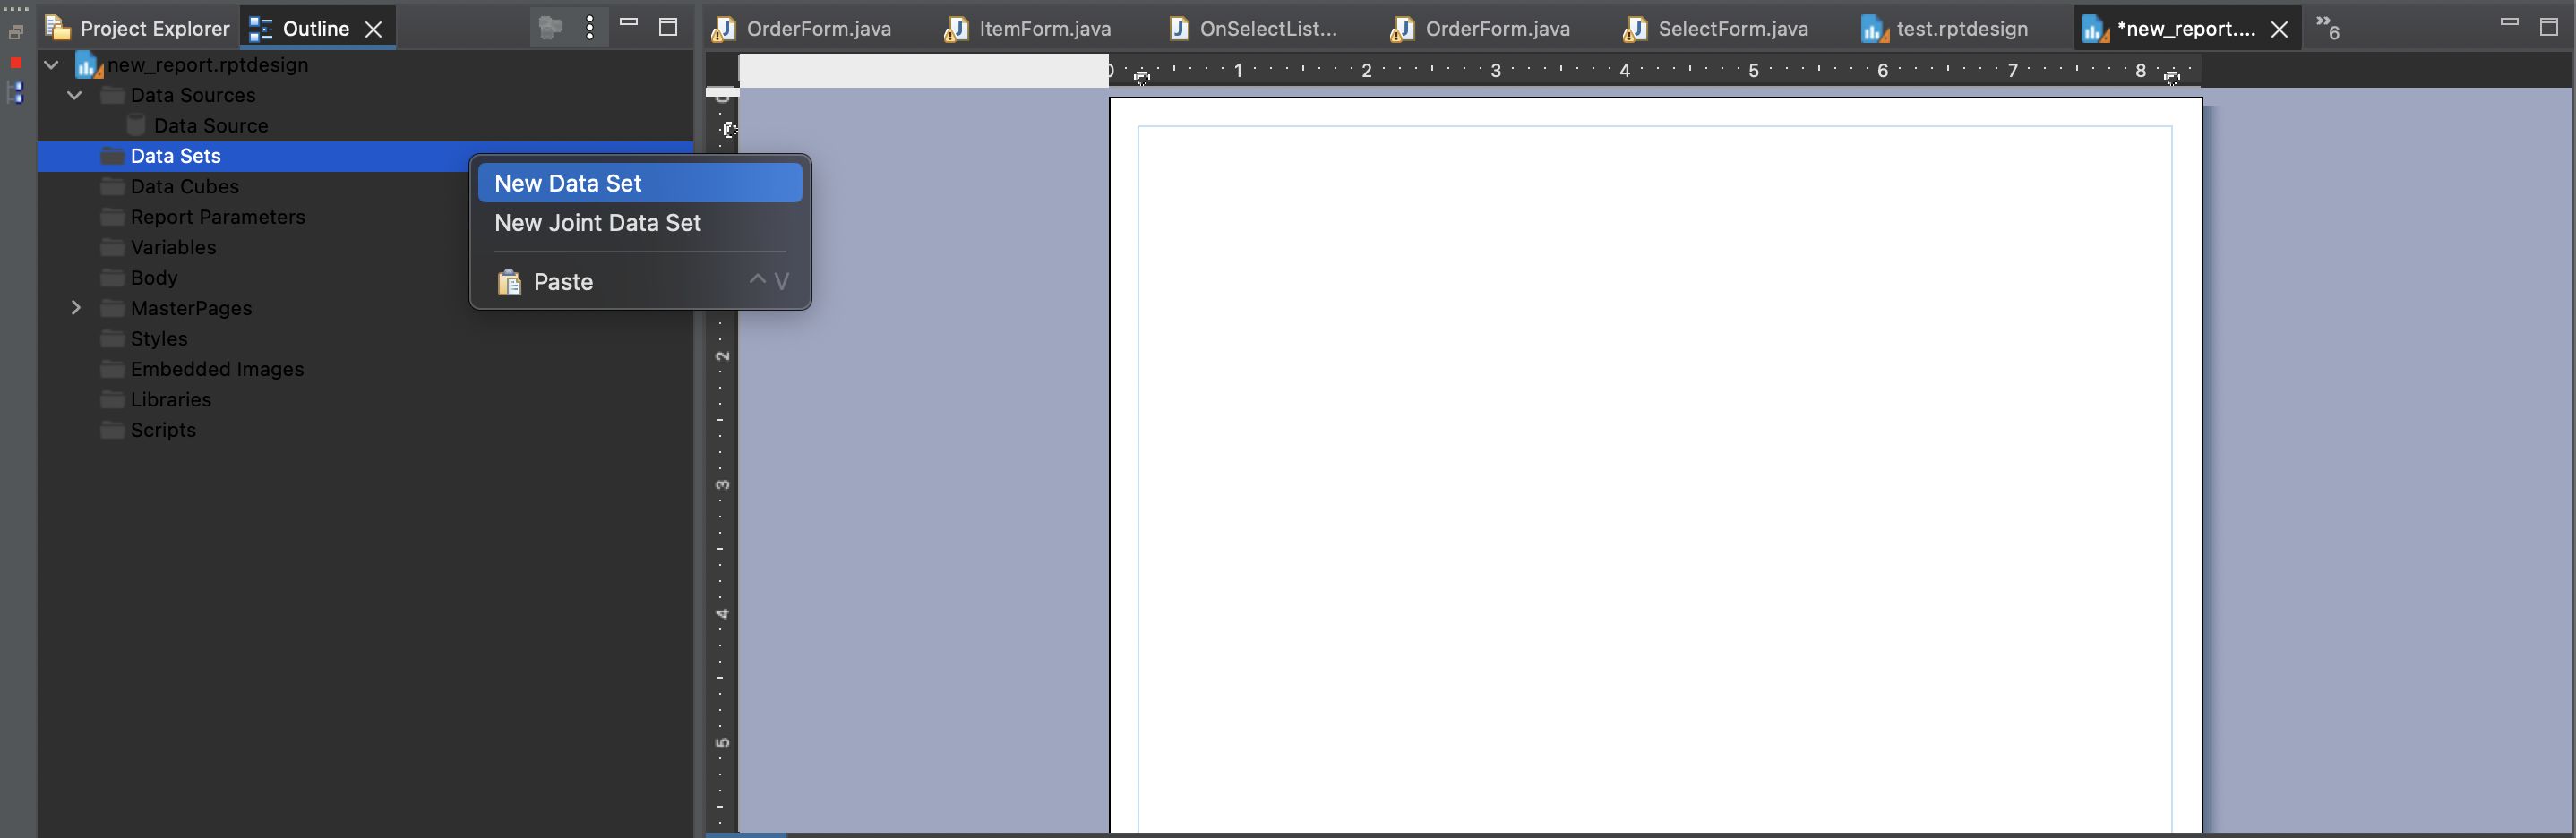
\includegraphics[width=0.5\textwidth]{assets/pertemuan14/Data-Set/birt-pre-new-data-set.png}
	
	\item Di dalam \textit{New Data Set Wizard}, berikan nama untuk \textit{Data Set} baru Anda.
	
	\item Pilih \textit{Data Source} yang terhubung ke database JDBC Anda.
	
	\item Pilih \textbf{SQL Select Query} sebagai tipe \textit{Data Set} dan klik \textbf{Next}. \\
	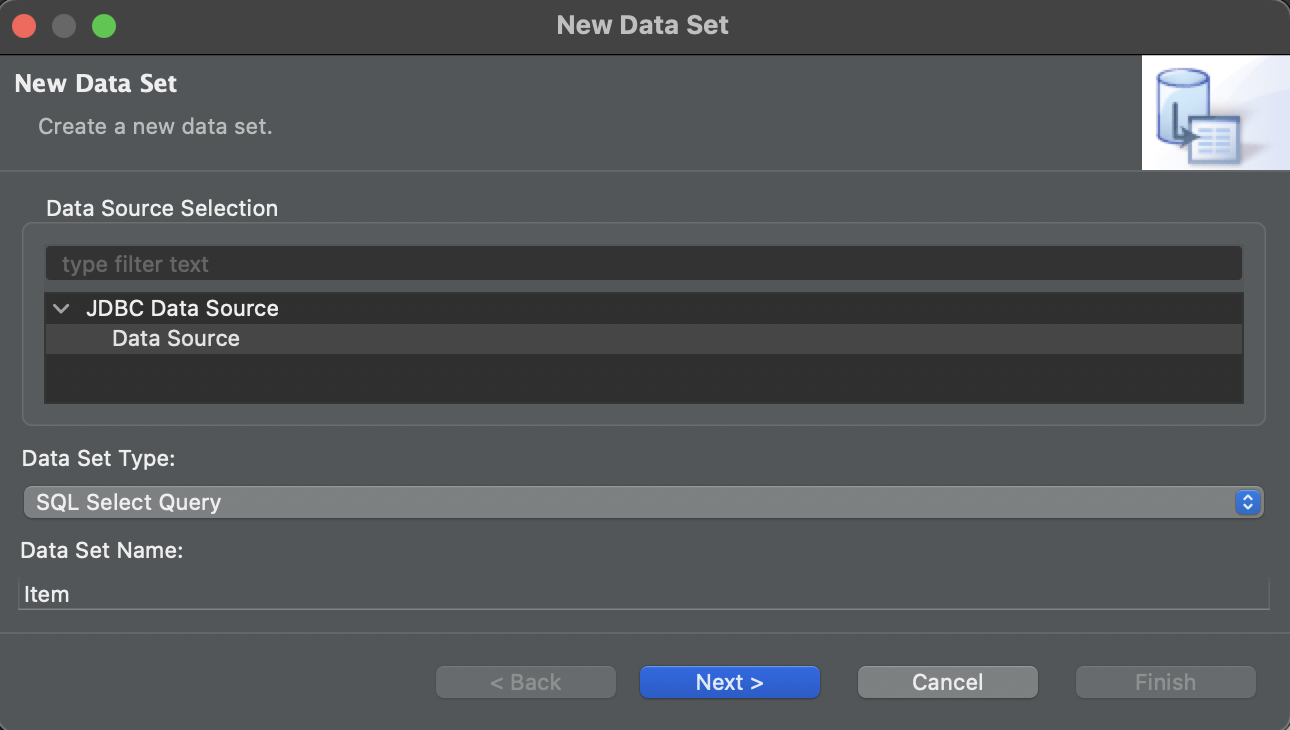
\includegraphics[width=0.5\textwidth]{assets/pertemuan14/Data-Set/birt-new-data-set.png}
	
	
	\item Pada tampilan Edit Data Set, pilih section Query \\
	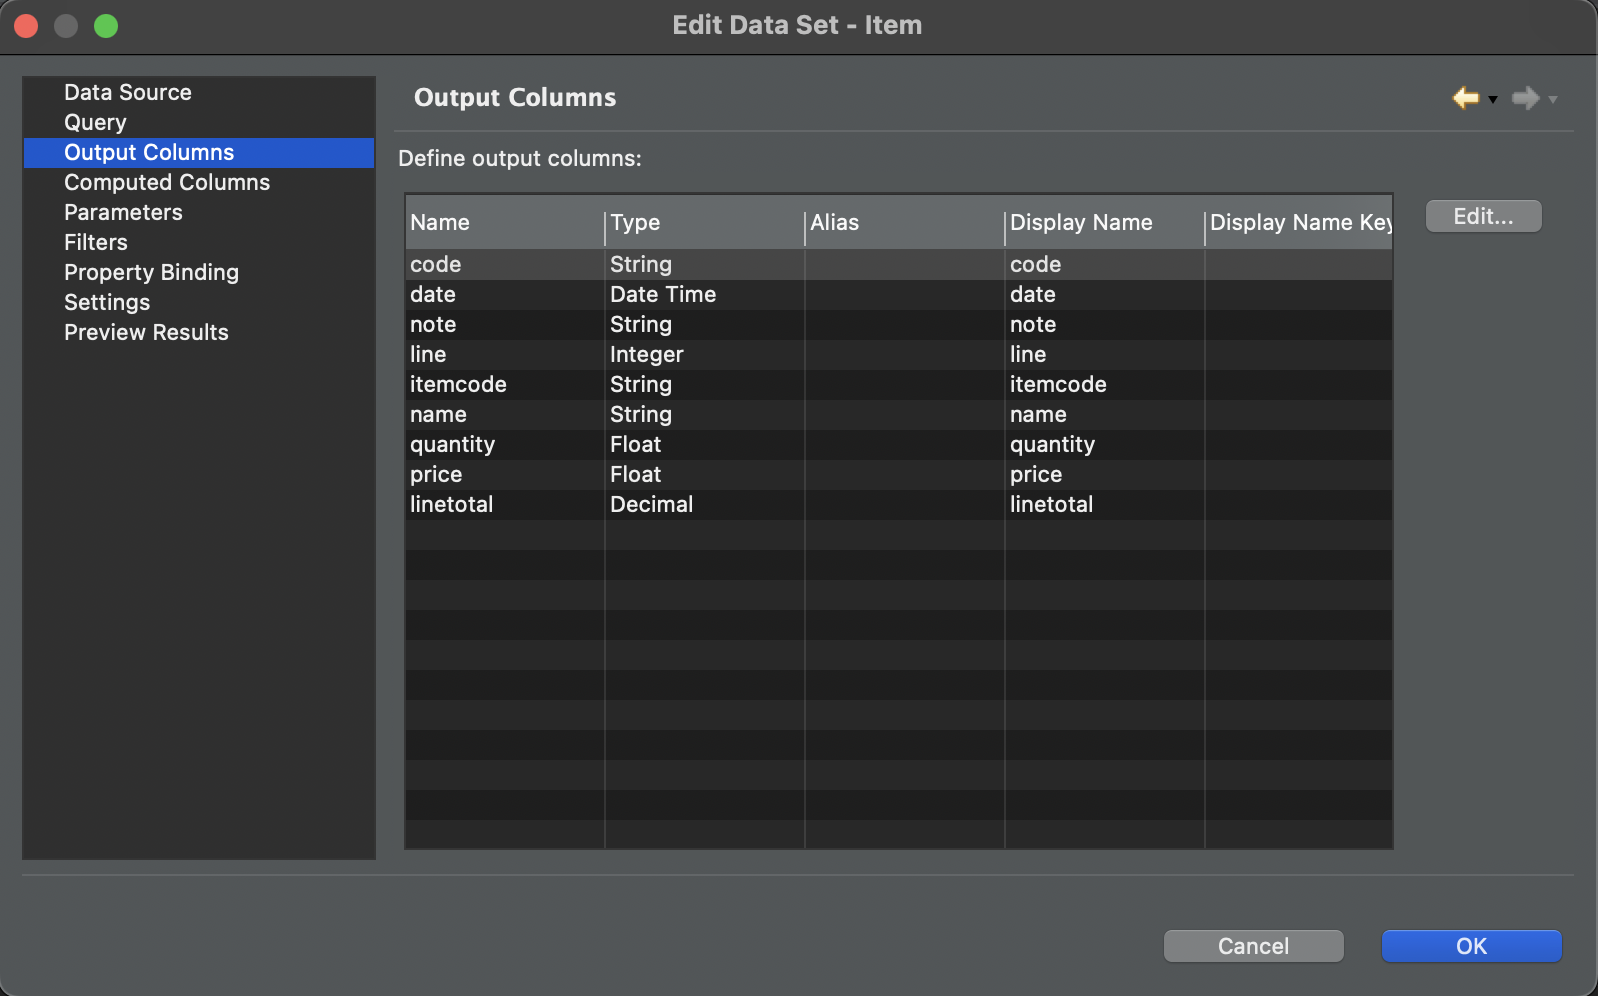
\includegraphics[width=0.8\textwidth]{assets/pertemuan14/Data-Set/birt-edit-data-set.png}
	
	\item Masukkan pernyataan SQL (\textit{SQL query}) yang ingin Anda gunakan untuk mengambil data. Misalnya:
	\begin{lstlisting}[style=JavaStyle]
			select 
				t1.code, t1.date, t1.note, 
				t2.line, t2.itemcode, t2.name, 
				t2.quantity, t2.price, 
				(t2.quantity * t2.price) linetotal
			from 
				`order` t1, order_detail t2 
			where 
				t1.code = t2.code
				and t1.code = ?
			order by 
				t1.code, t2.line;
		\end{lstlisting} 
		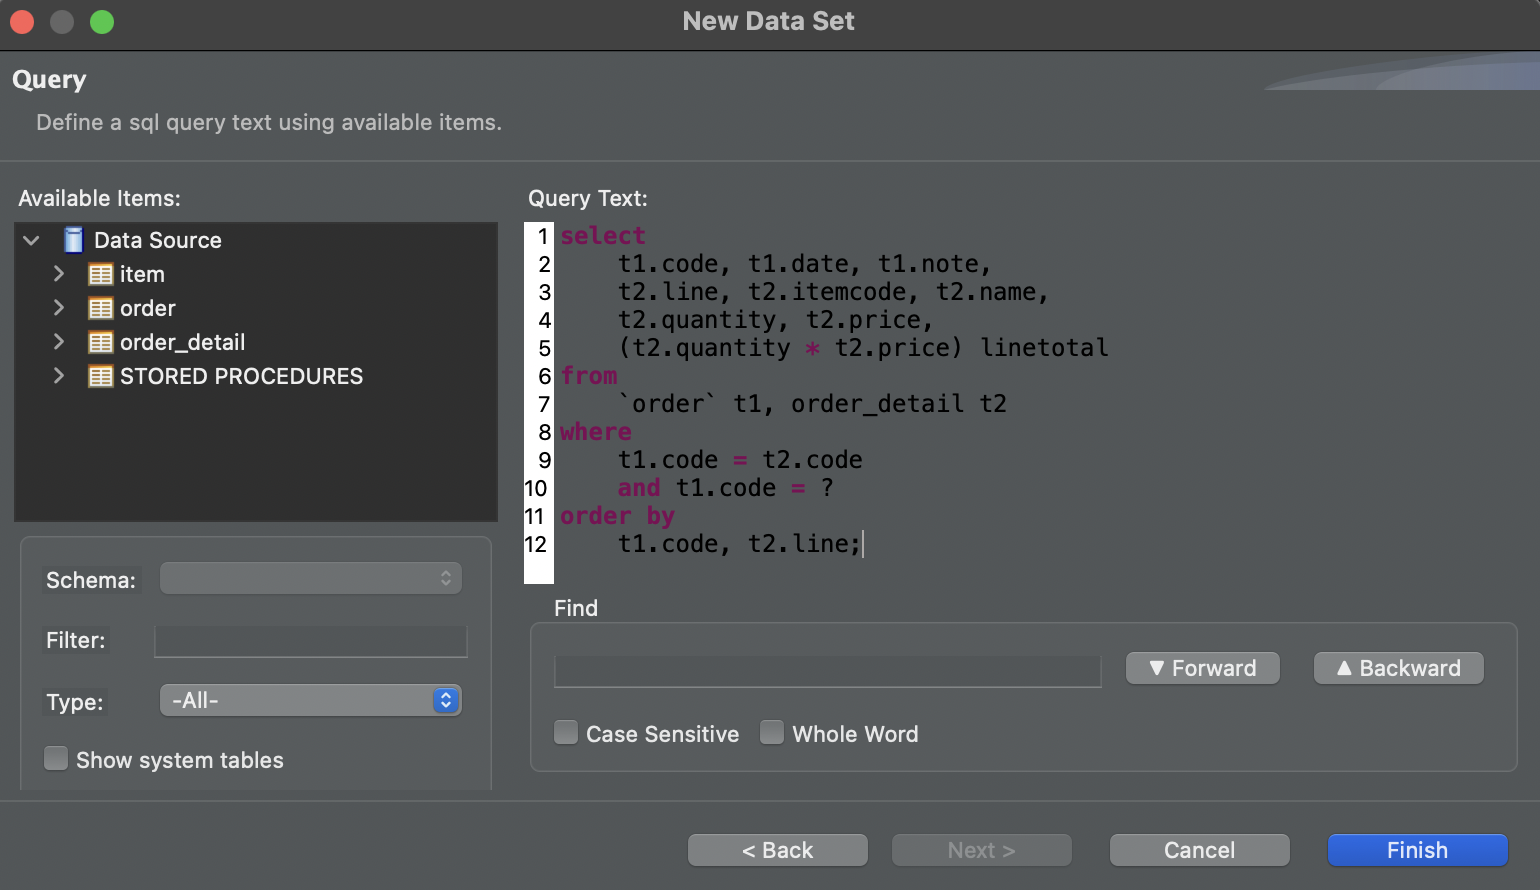
\includegraphics[width=0.8\textwidth]{assets/pertemuan14/Data-Set/birt-query.png}
	
	\item Klik \textbf{Finish} untuk menyimpan \textit{Data Set} yang baru.
	
	\item Bila ada warning seperti dibawah ini, abaikan saja terlebih dahulu karena akan ditambahkan pada langkah selanjutnya. \\
	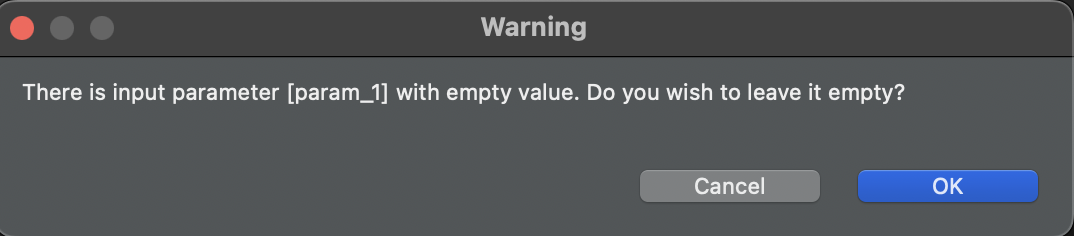
\includegraphics[width=0.8\textwidth]{assets/pertemuan14/Data-Set/birt-warning-after-data-set.png}
	
\end{enumerate}

\subsection{Menambah atau Mengedit Parameter}

Parameter memungkinkan pengguna untuk memasukkan nilai-nilai tertentu yang dapat mempengaruhi tampilan atau isi laporan. Berikut adalah langkah-langkah untuk menambah atau mengedit parameter:

\begin{enumerate}
	\item Klik kanan pada \textbf{Report Parameters} dan pilih \textbf{New Parameter}. \\
	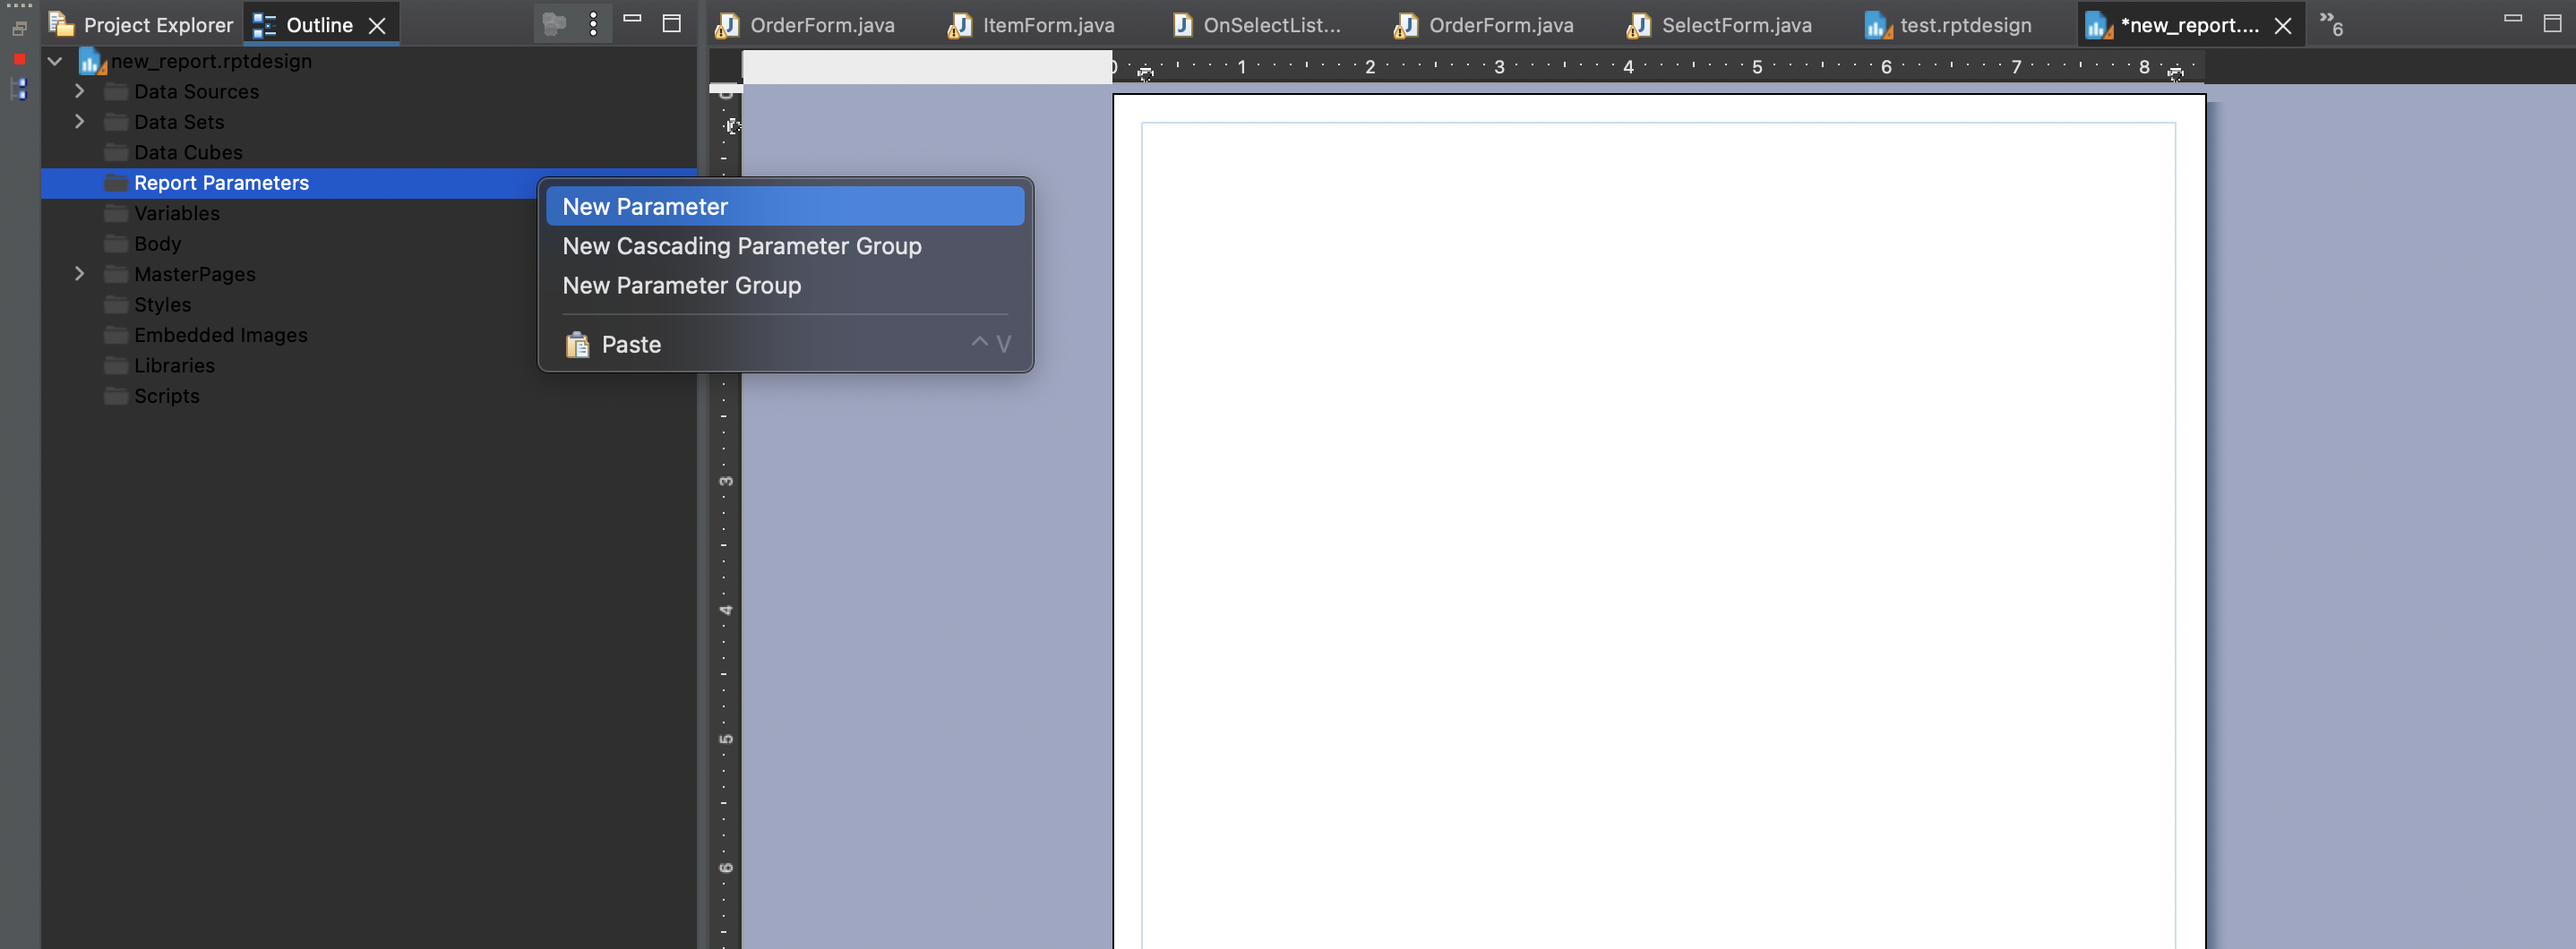
\includegraphics[width=0.8\textwidth]{assets/pertemuan14/Parameters/birt-pre-report-parameters.png}
	
	\item Masukkan nama parameter dan tentukan tipe datanya seperti gambar dibawah ini. \\
	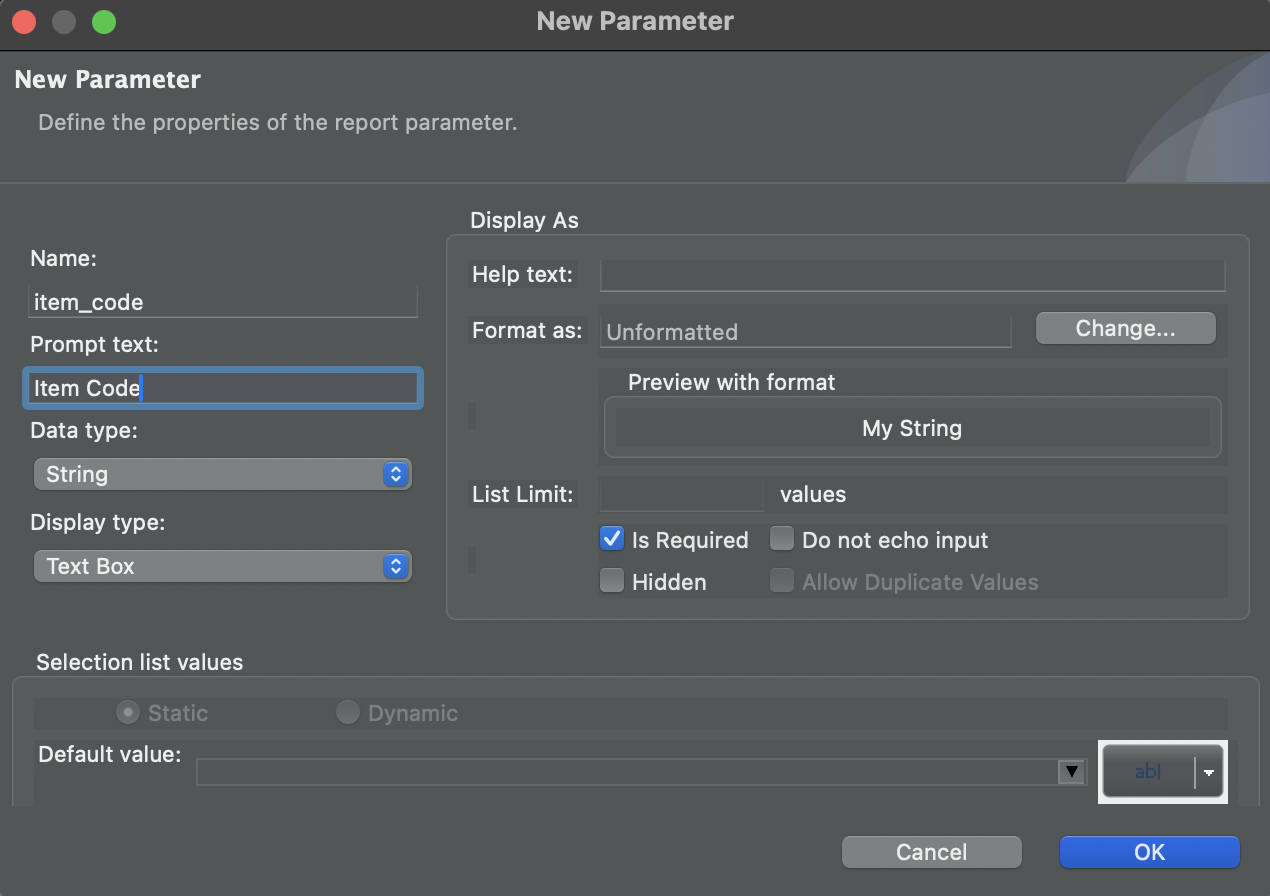
\includegraphics[width=0.8\textwidth]{assets/pertemuan14/Parameters/birt-new-parameter.png}

	\item Untuk mengedit parameter yang sudah ada, klik kanan pada datasets yang sudah ditambahkan sebelumnya, kemudian pilih Edit. \\
	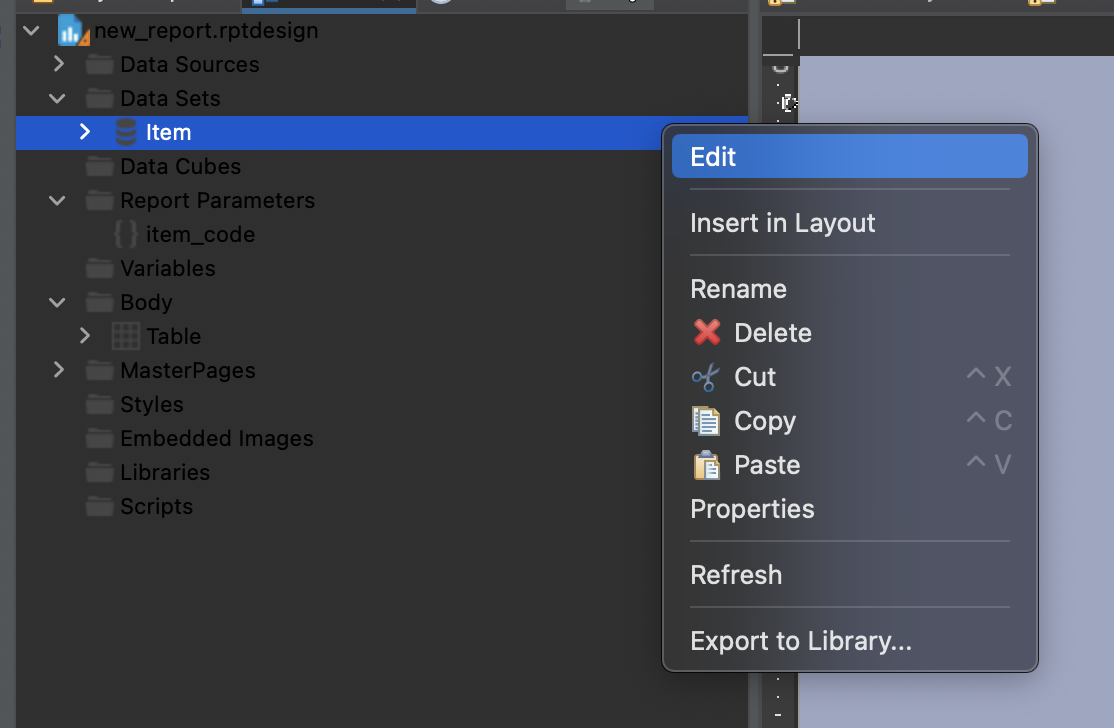
\includegraphics[width=0.8\textwidth]{assets/pertemuan14/Parameters/birt-edit-data-set.png}
	
	\item Pilih section parameters. 
	
	\item Pilih \textbf{params\_1}, kemudian klik Edit \\
	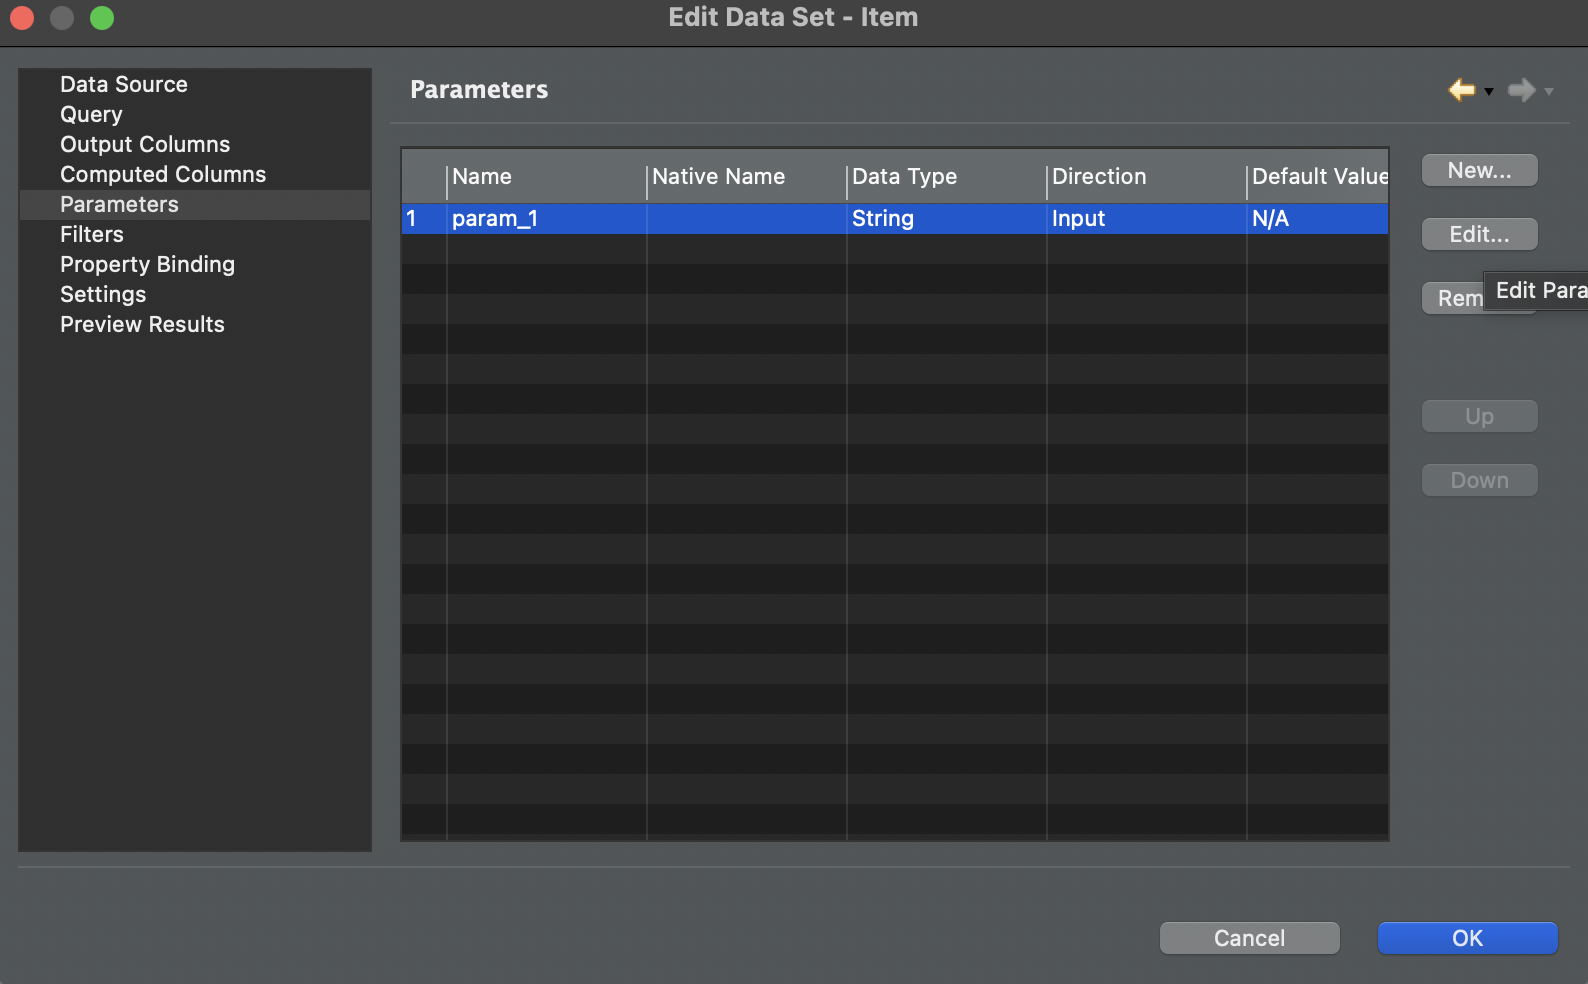
\includegraphics[width=0.8\textwidth]{assets/pertemuan14/Parameters/birt-edit-data-set-edit-parameters.png}
	
	\item Pada tampilan edit parameters, buatlah menjadi persis seperti gambar dibawah. Lalu klik \textbf{OK} untuk menyimpan pengaturan parameter. \\
	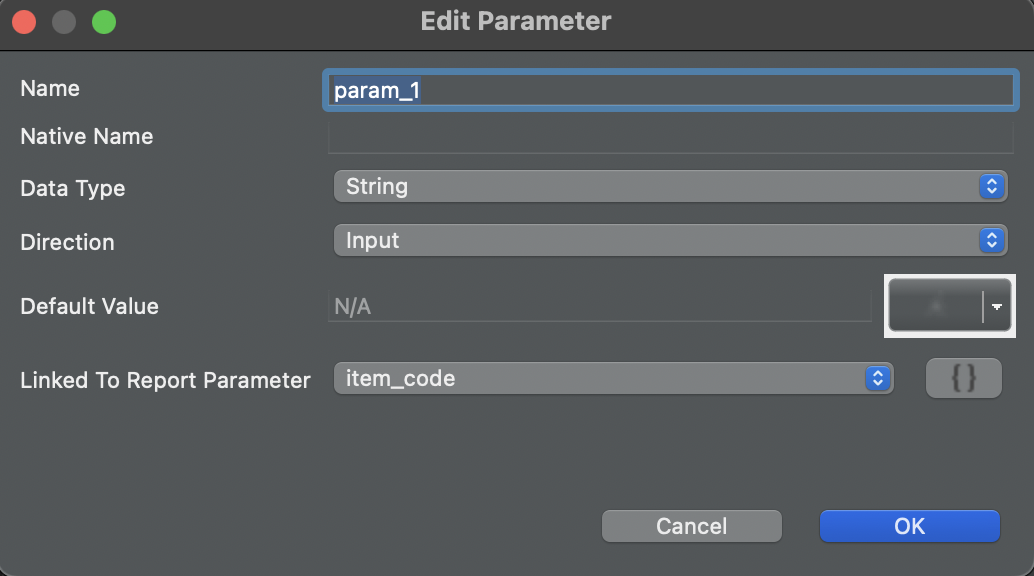
\includegraphics[width=0.8\textwidth]{assets/pertemuan14/Parameters/birt-edit-parameter.png}
	
	\item Bila muncul tampilan seperti ini, Pilih Yes \\
	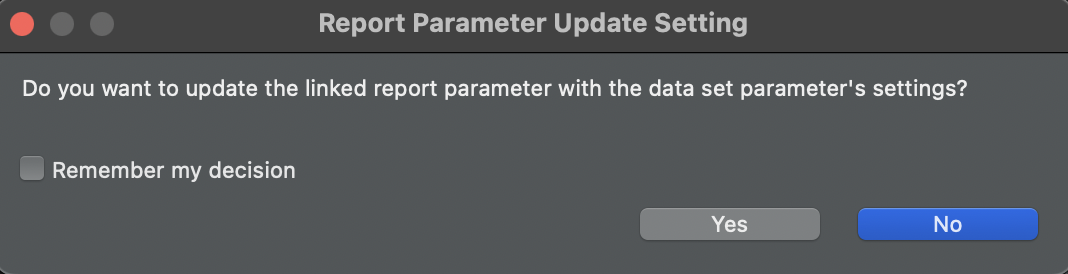
\includegraphics[width=0.8\textwidth]{assets/pertemuan14/Parameters/birt-report-parameter-update-settings.png}
	
\end{enumerate}

\section{Contoh Kode}

Studi kasus sama dengan pertemuan 12

\subsection{Kode SQL (pradita.sql)}

\begin{lstlisting}[style=JavaStyle]
	use pradita;
	
	delete from order_detail where code <> '';
	delete from `order` where code <> '';
	delete from item where code <> '';
	
	insert into item(code, name, quantity, price) values('IM001', 'Indomie Goreng', 30, 4100);
	insert into item(code, name, quantity, price) values('IM002', 'Indomie Kuah', 20, 4000);
	
	insert into `order`(code, note) values('1000000001', 'Penjualan Pertama');
	insert into order_detail(code, line, itemcode, name, quantity, price) 
	values('1000000001', 1, 'IM001', 'Indomie Goreng', 1, 4100);
	insert into order_detail(code, line, itemcode, name, quantity, price) 
	values('1000000001', 2, 'IM002', 'Indomie Kuah', 2, 4000);
	
	insert into `order`(code, note) values('1000000002', 'Penjualan Kedua');
	insert into order_detail(code, line, itemcode, name, quantity, price) 
	values('1000000002', 1, 'IM001', 'Indomie Goreng', 2, 4100);
	
	insert into `order`(code, note) values('1000000003', 'Penjualan Ketiga');
	insert into order_detail(code, line, itemcode, name, quantity, price) 
	values('1000000003', 1, 'IM002', 'Indomie Kuah', 4, 4000);
	
	select t1.code, t1.date, t1.note, t2.line, t2.itemcode, t2.name, t2.quantity, t2.price, 
	(t2.quantity * t2.price) linetotal
	from `order` t1, order_detail t2 where t1.code = t2.code;
\end{lstlisting}


\subsection{Kode SQL (crud.sql)}

\begin{lstlisting}[style=JavaStyle]
	# first
	select * from `order` t1 where t1.code = (select min(code)  from `order` t2) limit 1;
	
	# previous
	select * from `order` t1 where t1.code = (select max(code)  from `order` t2 where t2.code < 'TA00000002') limit 1;
	
	# next
	select * from `order` t1 where t1.code = (select min(code)  from `order` t2 where t2.code > 'TA00000002') limit 1;
	
	# last
	select * from `order` t1 where t1.code = (select max(code)  from `order` t2) limit 1;
	select line, itemcode, name, quantity, price, (quantity * price) total from `order_detail` t1 where t1.code = (select max(code)  from `order` t2);
	
	#get the last code
	SELECT Max(code) code FROM `order`
\end{lstlisting}


\subsection{Kode Java (OnSelectListener.java)}

\begin{lstlisting}[style=JavaStyle]
	package edu.pradita.p14;
	
	public interface OnSelectListener {
			
			public void select(Object[] values);
		}
\end{lstlisting}

\subsection{Kode Java (SelectForm.java)}

Sama persis dengan pertemuan 13

\begin{lstlisting}[style=JavaStyle]
	package edu.pradita.p14;
	
	import java.awt.BorderLayout;
	import java.awt.EventQueue;
	
	import javax.swing.JFrame;
	import javax.swing.JPanel;
	import javax.swing.border.EmptyBorder;
	import java.awt.Font;
	import java.awt.GraphicsEnvironment;
	
	import javax.swing.JLabel;
	import javax.swing.JTextField;
	import javax.swing.JTable;
	import javax.swing.JScrollPane;
	import javax.swing.table.DefaultTableModel;
	import javax.swing.table.TableColumn;
	import javax.swing.JButton;
	import javax.swing.BoxLayout;
	import java.awt.Component;
	import java.awt.GridLayout;
	import javax.swing.SwingConstants;
	import java.awt.GridBagLayout;
	import java.awt.GridBagConstraints;
	import java.awt.Insets;
	import java.awt.Point;
	
	import javax.swing.ListSelectionModel;
	import java.awt.event.ActionListener;
	import java.sql.PreparedStatement;
	import java.sql.ResultSet;
	import java.sql.ResultSetMetaData;
	import java.sql.SQLException;
	import java.awt.event.ActionEvent;
	import java.awt.Window.Type;
	
	public class SelectForm extends JFrame {
			
			private JPanel contentPane;
			private JTable table;
			private JTextField textField;
			private OnSelectListener onSelectListener = new OnSelectListener() {
					@Override
					public void select(Object[] values) {
						}
				};
			private String query;
			
			/**
			* Create the frame.
			*/
			public SelectForm(String query) {
					setAlwaysOnTop(true);
					setType(Type.UTILITY);
					setTitle("Select Form");
					setFont(new Font("Tahoma", Font.PLAIN, 16));
					setDefaultCloseOperation(JFrame.DISPOSE_ON_CLOSE);
					setBounds(100, 100, 350, 270);
					contentPane = new JPanel();
					contentPane.setBorder(new EmptyBorder(5, 5, 5, 5));
					setContentPane(contentPane);
					contentPane.setLayout(new BorderLayout(0, 4));
					
					Point centerPoint = GraphicsEnvironment.getLocalGraphicsEnvironment().getCenterPoint();
					this.setLocation(centerPoint.x - (int) this.getSize().getWidth() / 2,
					centerPoint.y - (int) this.getSize().getHeight() / 2);
					
					JPanel panel = new JPanel();
					contentPane.add(panel, BorderLayout.SOUTH);
					panel.setLayout(new GridLayout(1, 2, 0, 0));
					
					JButton btnCancel = new JButton("Cancel");
					btnCancel.addActionListener(new ActionListener() {
							public void actionPerformed(ActionEvent e) {
									SelectForm.this.setVisible(false);
									SelectForm.this.dispose();
								}
						});
					btnCancel.setAlignmentX(Component.CENTER_ALIGNMENT);
					btnCancel.setAlignmentY(Component.BOTTOM_ALIGNMENT);
					btnCancel.setFont(new Font("Tahoma", Font.PLAIN, 16));
					panel.add(btnCancel);
					
					JScrollPane scrollPane = new JScrollPane();
					contentPane.add(scrollPane, BorderLayout.CENTER);
					
					table = new JTable();
					table.setFont(new Font("Tahoma", Font.PLAIN, 16));
					table.setSelectionMode(ListSelectionModel.SINGLE_SELECTION);
					table.setModel(
					new DefaultTableModel(new Object[][] { { null, null }, }, new String[] { "Code", "Description" }) {
							private static final long serialVersionUID = 1L;
							Class[] columnTypes = new Class[] { String.class, String.class };
							
							public Class getColumnClass(int columnIndex) {
									return columnTypes[columnIndex];
								}
							
							boolean[] columnEditables = new boolean[] { false, false };
							
							public boolean isCellEditable(int row, int column) {
									return columnEditables[column];
								}
						});
					table.getColumnModel().getColumn(0).setPreferredWidth(71);
					table.getColumnModel().getColumn(1).setPreferredWidth(204);
					scrollPane.setViewportView(table);
					
					JPanel panel_1 = new JPanel();
					contentPane.add(panel_1, BorderLayout.NORTH);
					panel_1.setLayout(new BorderLayout(10, 0));
					
					JLabel lblFind = new JLabel("Find:");
					lblFind.setFont(new Font("Tahoma", Font.PLAIN, 16));
					panel_1.add(lblFind, BorderLayout.WEST);
					
					textField = new JTextField();
					lblFind.setLabelFor(textField);
					textField.setFont(new Font("Tahoma", Font.PLAIN, 16));
					textField.setColumns(10);
					panel_1.add(textField);
					
					JButton btnFind = new JButton("Find");
					btnFind.setFont(new Font("Tahoma", Font.PLAIN, 16));
					panel_1.add(btnFind, BorderLayout.EAST);
					
					JButton btnSelect = new JButton("Select");
					btnSelect.addActionListener(new ActionListener() {
							public void actionPerformed(ActionEvent e) {
									DefaultTableModel dtm = (DefaultTableModel) table.getModel();
									int row = table.getSelectedRow();
									int colCount = dtm.getColumnCount();
									Object[] values = new Object[colCount];
									for (int col = 0; col < dtm.getColumnCount(); col++) {
											Object val = dtm.getValueAt(row, col);
											values[col] = val;
										}
									SelectForm.this.onSelectListener.select(values);
									SelectForm.this.setVisible(false);
									SelectForm.this.dispose();
								}
						});
					
					btnSelect.setAlignmentX(Component.CENTER_ALIGNMENT);
					btnSelect.setFont(new Font("Tahoma", Font.PLAIN, 16));
					panel.add(btnSelect);
					
					try {
							this.query = query;
							PreparedStatement statement = OrderForm.CONNECTION.prepareStatement(query);
							ResultSet resultSet = statement.executeQuery();
							
							ResultSetMetaData metadata = resultSet.getMetaData();
							int colCount = metadata.getColumnCount();
							
							String[] columnNames = new String[colCount];
							for (int i = 1; i <= colCount; i++) {
									String colName = metadata.getColumnName(i);
									columnNames[i - 1] = colName;
								}
							
							Class<?>[] columnTypes = new Class<?>[colCount];
							for (int i = 0; i < colCount; i++) {
									columnTypes[i] = String.class;
								}
							
							boolean[] columnEditables = new boolean[colCount];
							for (int i = 0; i < colCount; i++) {
									columnEditables[i] = false;
								}
							
							DefaultTableModel dtm = new DefaultTableModel( //
							new Object[][] {}, // data
							columnNames // columns
							) {
									public Class getColumnClass(int columnIndex) {
											return columnTypes[columnIndex];
										}
									
									public boolean isCellEditable(int row, int column) {
											return columnEditables[column];
										}
								};
							
							// add the rows
							while (resultSet.next()) {
									Object[] values = new Object[colCount];
									for (int i = 1; i <= colCount; i++) {
											values[i - 1] = resultSet.getObject(i);
										}
									dtm.addRow(values);
								}
							resultSet.close();
							statement.close();
							
							table.setModel(dtm);
						} catch (SQLException e) {
							e.printStackTrace();
						}
					
				}
			
			public OnSelectListener getOnSelectListener() {
					return onSelectListener;
				}
			
			public void setOnSelectListener(OnSelectListener onSelectListener) {
					this.onSelectListener = onSelectListener;
				}
			
		}
\end{lstlisting}

\subsection{Kode Java (ItemForm.java)}

Direkomendasikan membuat form ini dengan WindowBuilder

\begin{lstlisting}[style=JavaStyle]
	package edu.pradita.p14;
	
	import java.awt.BorderLayout;
	import java.awt.EventQueue;
	
	import javax.swing.JFrame;
	import javax.swing.JPanel;
	import javax.swing.border.EmptyBorder;
	import java.awt.Font;
	import java.awt.GraphicsEnvironment;
	
	import javax.swing.JLabel;
	import javax.swing.JTextField;
	import javax.swing.JTable;
	import javax.swing.JScrollPane;
	import javax.swing.table.DefaultTableModel;
	import javax.swing.table.TableColumn;
	import javax.swing.JButton;
	import javax.swing.BoxLayout;
	import javax.swing.DefaultCellEditor;
	
	import java.awt.Component;
	import java.awt.GridLayout;
	import javax.swing.SwingConstants;
	import java.awt.GridBagLayout;
	import java.awt.GridBagConstraints;
	import java.awt.Insets;
	import java.awt.Point;
	
	import javax.swing.ListSelectionModel;
	import java.awt.event.ActionListener;
	import java.beans.PropertyChangeEvent;
	import java.beans.PropertyChangeListener;
	import java.sql.PreparedStatement;
	import java.sql.ResultSet;
	import java.sql.ResultSetMetaData;
	import java.sql.SQLException;
	import java.awt.event.ActionEvent;
	import java.awt.Window.Type;
	
	public class ItemForm extends JFrame {
		
		private JPanel contentPane;
		private JTable table;
		private String query;
		
		/**
		* Create the frame.
		*/
		public ItemForm() {
			setDefaultCloseOperation(JFrame.DISPOSE_ON_CLOSE);
			setAlwaysOnTop(true);
			setTitle("Item Form");
			setFont(new Font("Tahoma", Font.PLAIN, 16));
			setBounds(100, 100, 350, 270);
			contentPane = new JPanel();
			contentPane.setBorder(new EmptyBorder(5, 5, 5, 5));
			setContentPane(contentPane);
			contentPane.setLayout(new BorderLayout(0, 4));
			
			Point centerPoint = GraphicsEnvironment.getLocalGraphicsEnvironment().getCenterPoint();
			this.setLocation(centerPoint.x - (int) this.getSize().getWidth() / 2,
			centerPoint.y - (int) this.getSize().getHeight() / 2);
			
			JPanel panel = new JPanel();
			contentPane.add(panel, BorderLayout.SOUTH);
			panel.setLayout(new GridLayout(1, 2, 0, 0));
			
			JButton btnClose = new JButton("Close");
			btnClose.addActionListener(new ActionListener() {
				public void actionPerformed(ActionEvent e) {
					ItemForm.this.setVisible(false);
					ItemForm.this.dispose();
				}
			});
			btnClose.setAlignmentX(Component.CENTER_ALIGNMENT);
			btnClose.setAlignmentY(Component.BOTTOM_ALIGNMENT);
			btnClose.setFont(new Font("Tahoma", Font.PLAIN, 16));
			panel.add(btnClose);
			
			JScrollPane scrollPane = new JScrollPane();
			contentPane.add(scrollPane, BorderLayout.CENTER);
			
			table = new JTable();
			table.setFont(new Font("Tahoma", Font.PLAIN, 16));
			table.setSelectionMode(ListSelectionModel.SINGLE_SELECTION);
			table.setModel(new DefaultTableModel(new Object[][] { { null, null, null, null }, },
			new String[] { "Code", "Name", "Price", "Quantity" }) {
				Class[] columnTypes = new Class[] { String.class, String.class, Double.class, Double.class };
				
				public Class getColumnClass(int columnIndex) {
					return columnTypes[columnIndex];
				}
				
				boolean[] lastRowColumnEditables = new boolean[] { true, true, true, true };
				boolean[] columnEditables = new boolean[] { true, true, true, true };
				
				public boolean isCellEditable(int row, int column) {
					if (this.getRowCount() > 0 && row == this.getRowCount() - 1) {
						return lastRowColumnEditables[column];
					} else {
						return columnEditables[column];
					}
				}
			});
			table.getColumnModel().getColumn(0).setPreferredWidth(52);
			table.getColumnModel().getColumn(1).setPreferredWidth(157);
			table.getColumnModel().getColumn(3).setPreferredWidth(55);
			scrollPane.setViewportView(table);
			
			table.addPropertyChangeListener(new PropertyChangeListener() {
				
				String oldCode = null;
				
				@Override
				public void propertyChange(PropertyChangeEvent evt) {
					if ("tableCellEditor".equals(evt.getPropertyName()) && table.isEditing()) {
						int selectedRow = table.getSelectedRow();
						DefaultTableModel dtm = (DefaultTableModel) table.getModel();
						oldCode = (String) dtm.getValueAt(selectedRow, 0);
					}
					
					if (!"tableCellEditor".equals(evt.getPropertyName()) || table.isEditing()) {
						return;
					}
					
					DefaultCellEditor cellEditor = (DefaultCellEditor) evt.getOldValue();
					DefaultTableModel dtm = (DefaultTableModel) table.getModel();
					int selectedRow = table.getSelectedRow();
					int selectedCol = table.getSelectedColumn();
					
					
					String code = (selectedCol == 0)? (String) cellEditor.getCellEditorValue() : oldCode;
					;
					if (code == null || code.trim().length() == 0) {
						return;
					}
					
					String name = (String) dtm.getValueAt(selectedRow, 1);
					
					
					Object priceStr = (selectedCol == 2) ? cellEditor.getCellEditorValue() : dtm.getValueAt(selectedRow, 2);
					if (priceStr == null) {
						return;
					} else if (priceStr instanceof Double) {
						priceStr = priceStr.toString();
					}
					
					Object qtyStr = (selectedCol == 3) ? cellEditor.getCellEditorValue() : dtm.getValueAt(selectedRow, 3);
					if (qtyStr == null) {
						return;
					} else if (qtyStr instanceof Double) {
						qtyStr = qtyStr.toString();
					}
					
					double price = 0;
					double quantity = 0;
					
					try {
						price = Double.parseDouble(priceStr.toString());
						quantity = Double.parseDouble(qtyStr.toString());
					} catch (Exception exe) {
						return;
					}
					
					try {
						String query = "UPDATE item SET code = ?, name = ?, price = ?, quantity = ? " 
						+ " WHERE code = ?";
						PreparedStatement statement = OrderForm.CONNECTION.prepareStatement(query);
						statement.setString(1, code);
						statement.setString(2, name);
						statement.setDouble(3, price);
						statement.setDouble(4, quantity);
						statement.setString(5, oldCode);
						if (statement.executeUpdate() > 0) {
							System.out.println("Item " + code + " has been successfully updated.");
						}
						// If no update then try insert a new one.
						else {
							statement.close();
							query = "INSERT INTO item(code, name, price, quantity) VALUES(?, ?, ?, ?);";
							statement = OrderForm.CONNECTION.prepareStatement(query);
							statement.setString(1, code);
							statement.setString(2, name);
							statement.setDouble(3, price);
							statement.setDouble(4, quantity);
							if (statement.executeUpdate() > 0) {
								System.out.println("A new item " + code + " has been added.");
							}
							statement.close();
						}
						
					} catch (SQLException e) {
						e.printStackTrace();
					}
				}
				// ----
			});
			
			updateTable();
			
		}
		
		private void updateTable() {
			try {
				String query = "SELECT code, name, price, quantity FROM item";
				PreparedStatement statement = OrderForm.CONNECTION.prepareStatement(query);
				ResultSet resultSet = statement.executeQuery();
				
				DefaultTableModel dtm = (DefaultTableModel) table.getModel();
				while (dtm.getRowCount() > 0) {
					dtm.removeRow(0);
				}
				
				// add the rows
				while (resultSet.next()) {
					Object[] values = new Object[4];
					values[0] = resultSet.getString("code");
					values[1] = resultSet.getString("name");
					values[2] = resultSet.getDouble("price");
					values[3] = resultSet.getDouble("quantity");
					dtm.addRow(values);
				}
				Object[] values = new Object[4];
				dtm.addRow(values);
				
				resultSet.close();
				statement.close();
				
				table.setModel(dtm);
			} catch (SQLException e) {
				e.printStackTrace();
			}
		}
	}
	
\end{lstlisting}

\subsubsection{Deskripsi Kode}
Kode ini memiliki beberapa bagian utama:
\begin{itemize}
	\item Kelas \texttt{ItemForm} yang memperluas \texttt{JFrame} untuk menampilkan form item.
	\item Tabel \texttt{JTable} dengan \texttt{DefaultTableModel} yang menampilkan data item dalam kolom \texttt{Code}, \texttt{Name}, \texttt{Price}, dan \texttt{Quantity}.
	\item \texttt{ActionListener} untuk tombol \texttt{Close} yang menutup form.
	\item \texttt{PropertyChangeListener} untuk mendeteksi perubahan data dalam tabel dan memperbarui basis data sesuai.
\end{itemize}

\subsection{Kode Java (OrderForm.java)}
	
	Note: "...." artinya tidak ada perubahan code dari yang sebelumnya, kode yang digunakan sama, hanya ada beberapa penambahan karena adanya fitur reporting
	
	\begin{lstlisting}[style=JavaStyle]
		....
		import javax.swing.JTable;
		import javax.swing.table.DefaultTableModel;
		
		import org.eclipse.birt.core.framework.Platform;
		import org.eclipse.birt.report.engine.api.EngineConfig;
		import org.eclipse.birt.report.engine.api.IReportEngine;
		import org.eclipse.birt.report.engine.api.IReportEngineFactory;
		import org.eclipse.birt.report.engine.api.IReportRunnable;
		import org.eclipse.birt.report.engine.api.IRunAndRenderTask;
		import org.eclipse.birt.report.engine.api.PDFRenderOption;
		
		import com.mysql.cj.x.protobuf.MysqlxDatatypes.Array;
		import javax.swing.JButton;
		
		....
		
		import java.beans.PropertyChangeEvent;
		import java.beans.PropertyChangeListener;
		import java.io.File;
		import java.math.BigDecimal;
		import java.awt.event.ActionListener;
		
		....
		
		import java.awt.event.ActionEvent;
		import javax.swing.JMenuBar;
		import javax.swing.JMenu;
		import javax.swing.JMenuItem;
		
		
		public class OrderForm {
			....
			private JButton btnDeleteItem;
			private JButton btnConfirm;
			private ItemForm itemForm;
			
			/**
			* Launch the application.
			.....
			
			/**
			* Initialize the contents of the frame.
			* 
			* @throws SQLException
			*/
			private void initialize() throws SQLException {
				....
				
				btnConfirm.addActionListener(new ActionListener() {
					public void actionPerformed(ActionEvent e) {
						
						PreparedStatement statement;
						try {
							// get max code
							statement = CONNECTION.prepareStatement("SELECT Max(code) code FROM `order`;");
							ResultSet resultSet = statement.executeQuery();
							String maxCode = null;
							if (resultSet.next()) {
								maxCode = resultSet.getString("code");
							}
							String newCode = String.valueOf(Integer.valueOf(maxCode) + 1);
							resultSet.close();
							statement.close();
							
							statement = CONNECTION.prepareStatement("insert into `order`(code, note) values(?, ?);");
							statement.setString(1, newCode);
							statement.setString(2, txtNote.getText());
							statement.executeUpdate();
							statement.close();
							
							for (int i = 0; i < table.getRowCount(); i++) {
								statement = CONNECTION
								.prepareStatement("insert into `order_detail`(code, line, itemcode, name, price, quantity)"
								+ " values(?, ?, ?, ?, ?, ?);");
								statement.setString(1, newCode);
								statement.setInt(2, (int) table.getValueAt(i, 0));
								statement.setString(3, (String) table.getValueAt(i, 1));
								statement.setString(4, (String) table.getValueAt(i, 2));
								statement.setDouble(5, Double.valueOf(table.getValueAt(i, 3).toString()));
								statement.setDouble(6, Double.valueOf(table.getValueAt(i, 4).toString()));
								statement.executeUpdate();
								
								// update the stock
								statement = CONNECTION.prepareStatement("UPDATE item SET quantity = quantity - ? " + "WHERE code = ?;");
								statement.setDouble(1, Double.valueOf(table.getValueAt(i, 4).toString()));
								statement.setString(2, (String) table.getValueAt(i, 1));
								statement.executeUpdate();
							}
							
							isAddMode = false;
							enableDisableElements();
							
							displayLastOrder();
						} catch (SQLException e1) {
							e1.printStackTrace();
						}
						
					}
				});
				
				.....
				
				txtNote = new JTextArea();
				txtNote.setRows(3);
				txtNote.setColumns(30);
				panel_4.add(txtNote);
				
				JMenuBar menuBar = new JMenuBar();
				frmOrderForm.setJMenuBar(menuBar);
				
				JMenu menuFile = new JMenu("File");
				menuFile.setMnemonic('F');
				menuBar.add(menuFile);
				
				JMenuItem menuItemPrint = new JMenuItem("Print");
				menuItemPrint.addActionListener(new ActionListener() {
					public void actionPerformed(ActionEvent e) {
						
						try {
							EngineConfig config = new EngineConfig();
							Platform.startup(config);
							final IReportEngineFactory FACTORY = (IReportEngineFactory) Platform
							.createFactoryObject(IReportEngineFactory.EXTENSION_REPORT_ENGINE_FACTORY);
							IReportEngine engine = FACTORY.createReportEngine(config);
							
							// Open the report design
							IReportRunnable design = null;
							design = engine.openReportDesign("reports/test.rptdesign");
							IRunAndRenderTask task = engine.createRunAndRenderTask(design);
							task.setParameterValue("order_code", txtCode.getText());
							task.validateParameters();
							
							PDFRenderOption options = new PDFRenderOption();
							options.setOutputFileName("reports/test.pdf");
							options.setOutputFormat("pdf");
							
							task.setRenderOption(options);
							task.run();
							task.close();
							engine.destroy();
							
							if (Desktop.isDesktopSupported()) {
								File myFile = new File("reports/test.pdf");
								Desktop.getDesktop().open(myFile);
							}
							
						} catch (Exception EX) {
							EX.printStackTrace();
						} finally {
							Platform.shutdown();
						}
						
					}
				});
				menuFile.add(menuItemPrint);
				
				JMenu menuMasterData = new JMenu("Master Data");
				menuMasterData.setMnemonic('M');
				menuBar.add(menuMasterData);
				
				JMenuItem menuItemItem = new JMenuItem("Item");
				menuItemItem.addActionListener(new ActionListener() {
					
					public void actionPerformed(ActionEvent e) {
						itemForm = new ItemForm();
						itemForm.setVisible(true);
					}
				});
				menuMasterData.add(menuItemItem);
				
				displayLastOrder();
				
			}
			
			....
			
			private void displayPrevOrder() {
				try {
					PreparedStatement statement = CONNECTION.prepareStatement(
					"select * from `order` t1 where t1.code = (select max(code)  from `order` t2 where t2.code < ?) limit 1;");
					String currentCode = txtCode.getText();
					statement.setString(1, currentCode);
					displayOrder(statement);
					isAddMode = false;
					enableDisableElements();
				} catch (SQLException e) {
					e.printStackTrace();
				}
			}
			
			private void displayNextOrder() {
				try {
					PreparedStatement statement = CONNECTION.prepareStatement(
					"select * from `order` t1 where t1.code = (select min(code)  from `order` t2 where t2.code > ?) limit 1;");
					String currentCode = txtCode.getText();
					statement.setString(1, currentCode);
					displayOrder(statement);
					isAddMode = false;
					enableDisableElements();
				} catch (SQLException e) {
					e.printStackTrace();
				}
			}
			
			private void displayLastOrder() {
				try {
					PreparedStatement statement = CONNECTION
					.prepareStatement("select * from `order` t1 where t1.code = (select max(code)  from `order` t2) limit 1");
					displayOrder(statement);
					isAddMode = false;
					enableDisableElements();
				} catch (SQLException e) {
					e.printStackTrace();
				}
			}
			
			private void displayOrder(PreparedStatement statement) throws SQLException {
				// initial order header query
				ResultSet resultSet = statement.executeQuery();
				if (resultSet.next()) {
					String code = resultSet.getString("code");
					txtCode.setText(code);
					txtDate.setText(resultSet.getString("date"));
					txtNote.setText(resultSet.getString("note"));
					resultSet.close();
					statement.close();
					
					// detail order detail query
					statement = CONNECTION.prepareStatement("select line, itemcode, name, price, quantity, (quantity * price) total "
					+ "from `order_detail` t1 where t1.code = ?");
					statement.setString(1, code);
					resultSet = statement.executeQuery();
					
					double grandTotal = 0;
					DefaultTableModel dtm = (DefaultTableModel) table.getModel();
					while (dtm.getRowCount() > 0) {
						dtm.removeRow(0);
					}
					while (resultSet.next()) {
						int line = resultSet.getInt("line");
						String itemcode = resultSet.getString("itemcode");
						String name = resultSet.getString("name");
						double quantity = resultSet.getInt("quantity");
						double price = resultSet.getInt("price");
						double total = resultSet.getInt("total");
						grandTotal = grandTotal + total;
						
						dtm.addRow(new Object[] { line, itemcode, name, price, quantity, total });
					}
					
					setTotalOrder(dtm);
				}
				
				resultSet.close();
				statement.close();
			}
			
			.....
\end{lstlisting}

		
\subsubsection{Penjelasan Kode Java pada \texttt{OrderForm.java}}

Kode \texttt{OrderForm.java} mengalami beberapa penambahan untuk mendukung fitur \textit{reporting}, khususnya dalam pembuatan laporan dalam format PDF menggunakan pustaka BIRT (Business Intelligence and Reporting Tools). Berikut adalah penjelasan dari bagian-bagian penting pada kode ini.

\begin{itemize}
	\item \textbf{Penambahan Impor Pustaka BIRT}:
	Kode mengimpor pustaka BIRT seperti \texttt{EngineConfig}, \texttt{IReportEngine}, \texttt{IReportEngineFactory}, \texttt{IReportRunnable}, dan \texttt{IRunAndRenderTask}. Pustaka-pustaka ini mendukung pembuatan dan pengaturan tugas untuk menghasilkan laporan dalam format PDF.
	
	\item \textbf{Penambahan Elemen pada Menu File}:
	Dibuat menu \texttt{File} pada bilah menu, dan di dalamnya terdapat opsi \texttt{Print} yang memungkinkan pengguna untuk mencetak laporan dalam format PDF. Ketika opsi ini dipilih, sebuah \textit{listener} akan memicu tugas pembuatan laporan.
	
	\item \textbf{Proses Membuat Laporan PDF}:
	\begin{itemize}
		\item \texttt{EngineConfig} diinisialisasi untuk konfigurasi mesin laporan BIRT.
		\item \texttt{IReportEngineFactory} digunakan untuk membuat \textit{instance} mesin laporan, dan \texttt{IReportRunnable} untuk memuat desain laporan.
		\item Sebuah \texttt{IRunAndRenderTask} dibuat berdasarkan desain laporan, kemudian parameter seperti \texttt{order\_code} diatur agar laporan sesuai dengan data pesanan.
		\item \texttt{PDFRenderOption} mengatur format keluaran menjadi PDF dan menentukan nama berkas hasil laporan.
		\item Setelah selesai, laporan dijalankan (\texttt{task.run()}) dan disimpan pada direktori tertentu.
	\end{itemize}
	
	\item \textbf{Menampilkan Laporan PDF}:
	Setelah laporan selesai, jika perangkat mendukung fungsi \textit{desktop}, berkas PDF akan otomatis dibuka di aplikasi pembaca PDF default.
	
	\item \textbf{Fitur Menampilkan Pesanan Terakhir}:
	Ditambahkan beberapa metode seperti \texttt{displayPrevOrder}, \texttt{displayNextOrder}, dan \texttt{displayLastOrder} yang memfasilitasi pengguna untuk melihat pesanan sebelumnya, berikutnya, dan terakhir.
	Dalam setiap metode, \texttt{PreparedStatement} digunakan untuk mengambil data dari database berdasarkan kode pesanan. Pesanan ditampilkan di layar dengan menyesuaikan elemen-elemen tampilan dan tabel.
	
	\item \textbf{Pembaharuan Tabel dengan Rincian Pesanan}:
	Dalam metode \texttt{displayOrder}, kode mengambil data pesanan dari tabel \texttt{order\_detail} dan mengisi tabel GUI dengan informasi seperti \textit{line item}, \textit{item code}, nama item, harga, jumlah, dan total biaya.
\end{itemize}

Secara keseluruhan, pembaruan ini mengintegrasikan fungsionalitas laporan PDF ke dalam aplikasi GUI, memungkinkan pengguna mencetak laporan pesanan dengan mudah, serta menambahkan kemampuan untuk menavigasi antar pesanan.



